\section{Common rules}
\label{sec:Common_rules}
The 5 vs. 5 games played at the GORE 2021 are designed to use the rules of RoboCup SPL as published in 2020. However, to facilitate the remote participation of all teams and the common robot pool, various changes are required.

Therefore, the following re-produces the rules from RoboCup SPL 2020, with various details that have been modified, added and/or omitted. Changes are marked with a \cbw{colourbox}.

\subsection{Setup of the Environment}
\label{sec:environment_setup}
\subsubsection{Field Construction (standard and minimum size)}
\label{sec:field_dim}

The \cbw{standard} soccer field consists of green 8mm artificial turf mounted on a flat wooden base with \cbw{outer field line dimensions of 9m x 6m and} a total area of length \TotalLength and width \TotalWidth. \cbw{This is termed the \textbf{standard SPL field}.} Care should be taken to ensure the field is as flat and level as possible.  Additionally, the wooden base should be well supported and should not give when humans stand or walk on it.

\cbp{To avoid the need for hosting teams to construct new fields for the GORE 2021, fields with outer field line dimensions of at least 6m x 4m can be used. Goal dimensions should still be the same as the standard size field. This setup is termed the \textbf{minimum size field}.}

The \cbw{standard} dimensions of the soccer field are shown in Figure~\ref{fig:field_dim}. A more detailed technical drawing is provided in Appendix~\ref{apx:technical-drawing} to this document.
Note that the penalty cross is a cross and there is a dash at centre field. White field lines can be made of the same 8mm artificial turf, but in white (\ie, made of white artificial turf), spray painted or taped. Regardless of the solution, the field lines must be durable throughout the competition.

The construction and placement of the goals is depicted in Figure~\ref{fig:goal_dimensions} and Figure~\ref{fig:goal_appearance}. The support structure for the net shall be made with small black, white, or grey bars or cylinders. The support structure shall be constructed exactly as shown in Figure \ref{fig:goal_appearance}.


\begin{figure}[b!]
	\centering
	\centerline{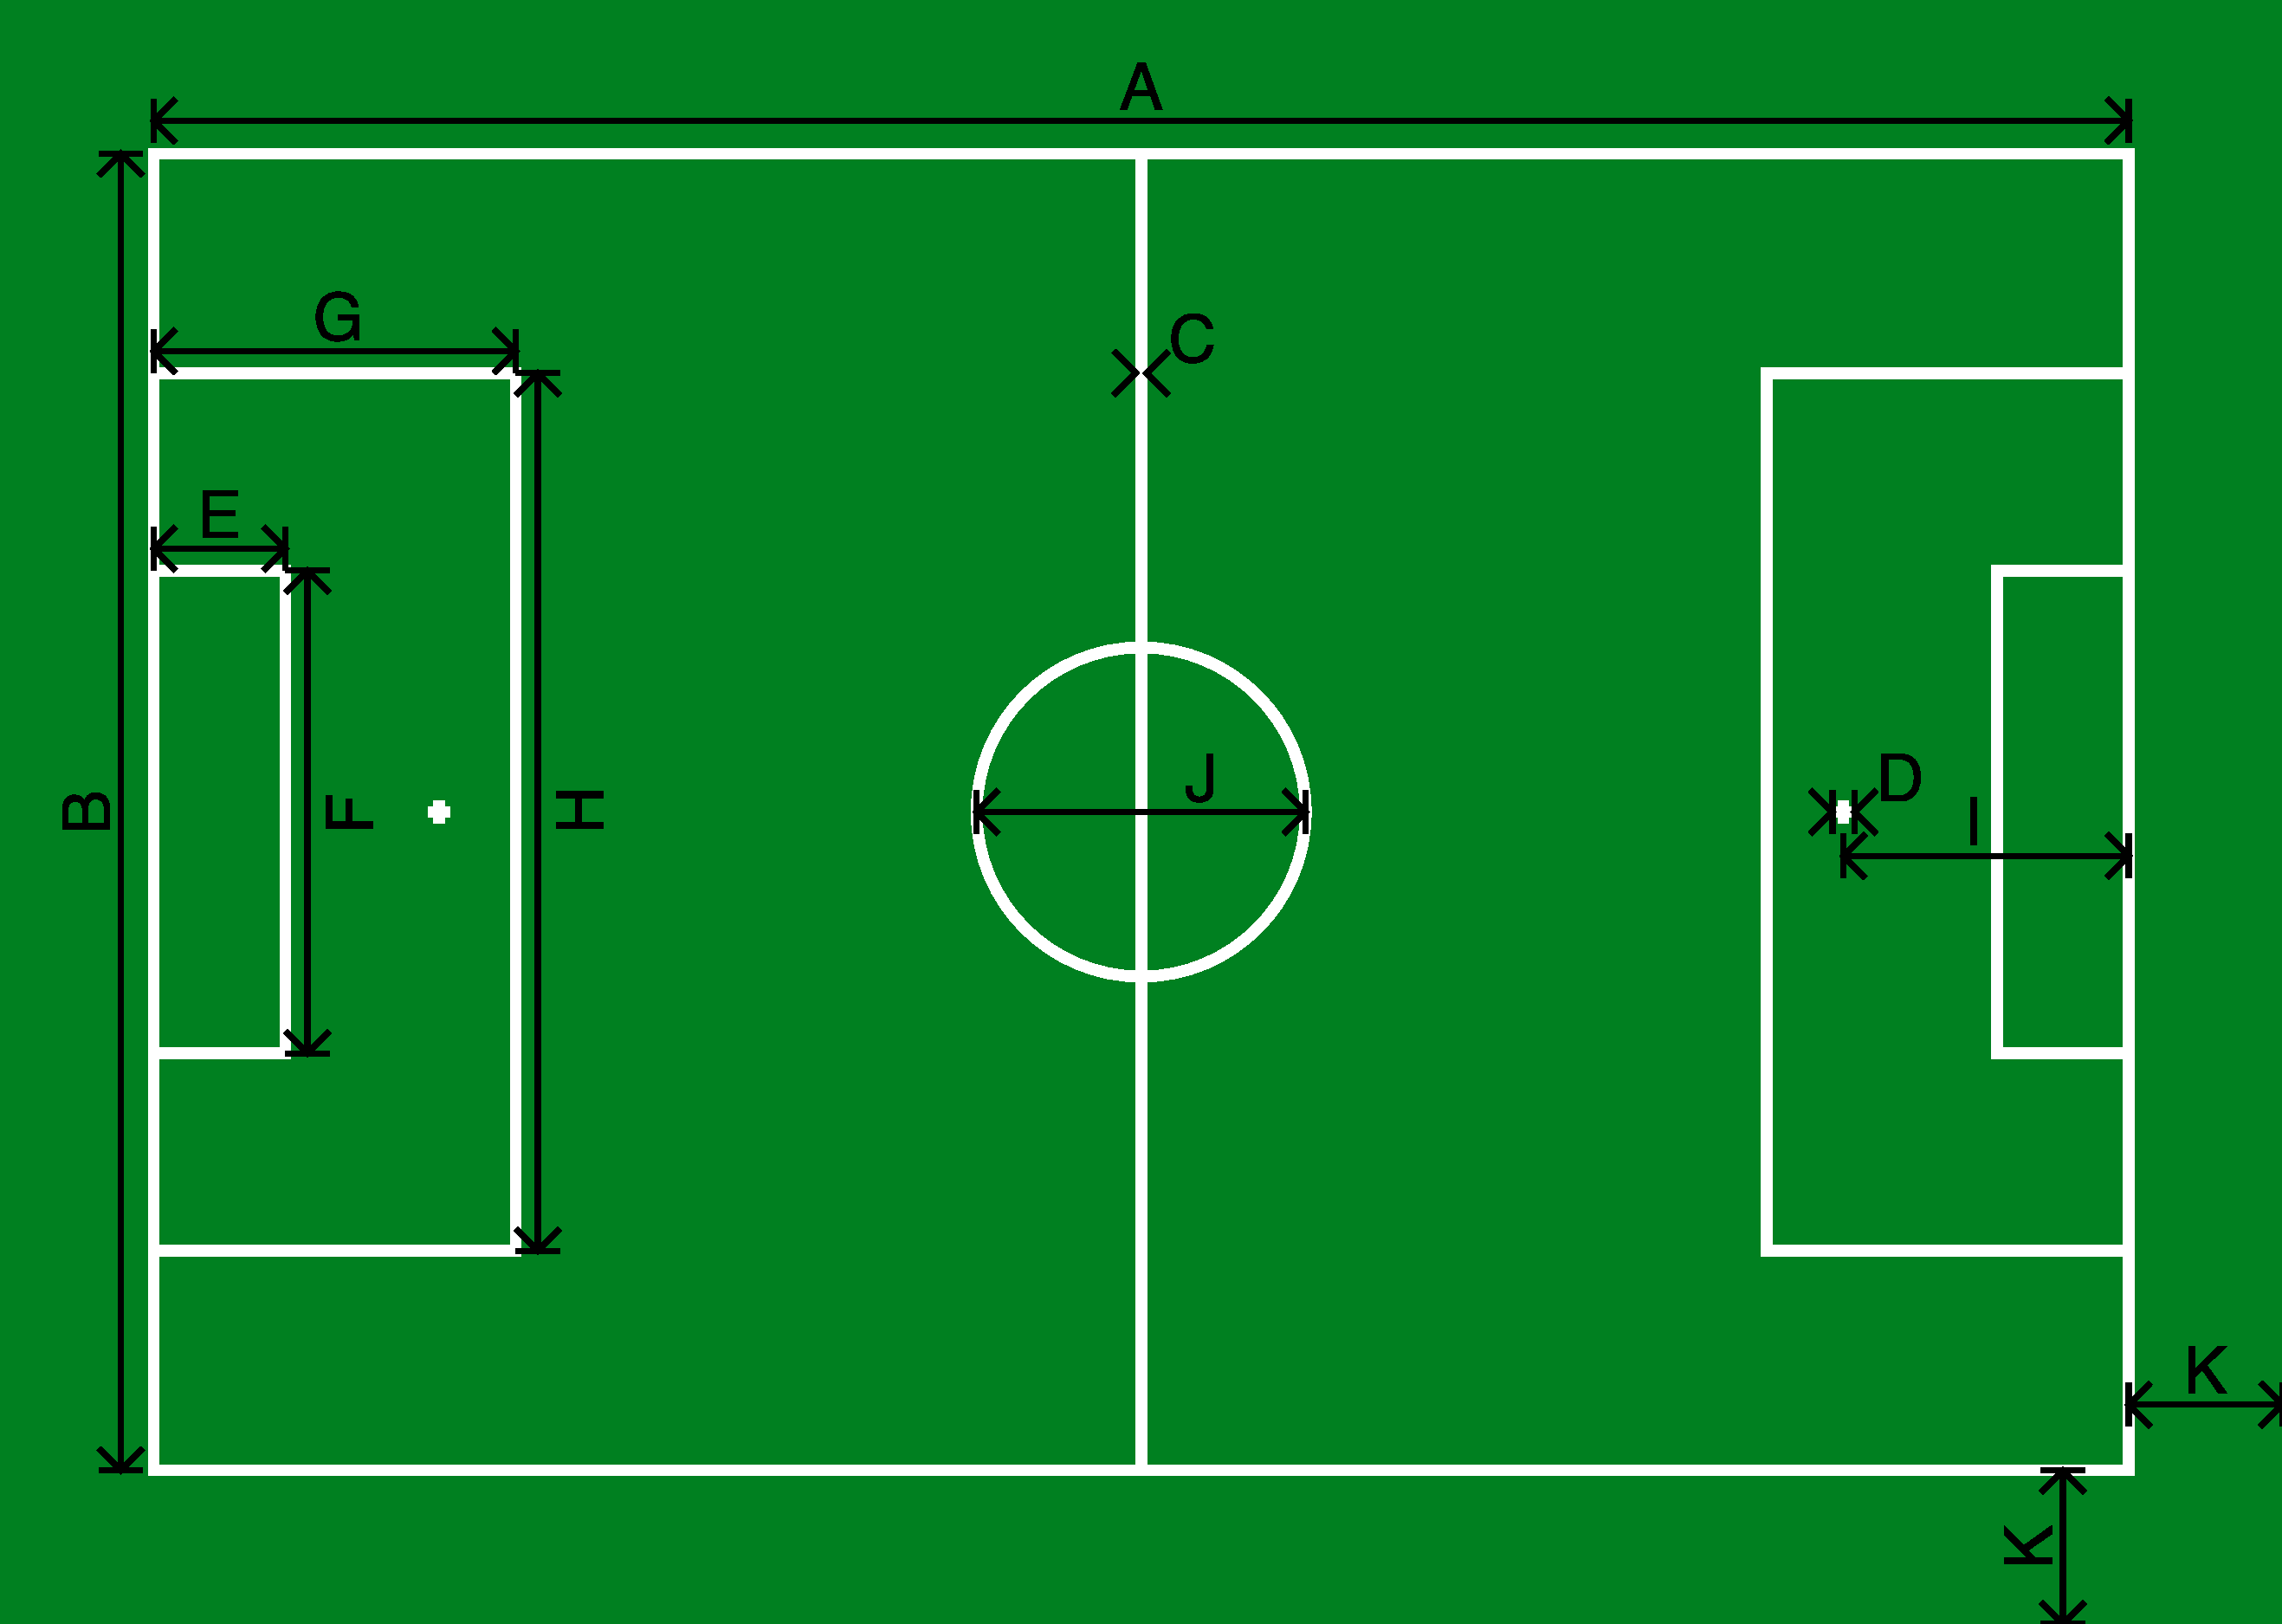
\includegraphics[width=\columnwidth]{figs/fieldDimensions2020.pdf}}
	\vspace{1ex}
	\begin{tabular}{| l | l | l |}
		ID & Description & Length (in mm) \\
		\hline \hline
		A & Field length & 9000 \\
		\hline
		B & Field width & 6000 \\
		\hline
		C & Line width & 50 \\
		\hline
		D & Penalty cross size & 100 \\
		\hline
		E & Goalbox area length & 600 \\
		\hline
		F & Goalbox area width & 2200 \\
	\end{tabular}
	\begin{tabular}{|l|l|l|}
		ID & Description & Length (in mm) \\
		\hline \hline
		G & Penalty area length & \cbw{1650} \\
		\hline
		H & Penalty area width & \cbw{4000} \\
		\hline
		I & Penalty cross distance & \cbw{1300} \\
		\hline
		J & Centre circle diameter & 1500 \\
		\hline
		K & Border strip width & 700 \\
		\hline
		&  &  \\
	\end{tabular}
	\caption{Schematic diagram of the  \cbw{standard} soccer field (not to scale) and corresponding dimensions in mm. Note that measurements on this diagram are made to the centre of lines.} \label{fig:field_dim}
\end{figure}


\begin{figure}[t!]
	\begin{center}
		\leavevmode
		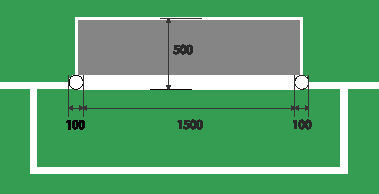
\includegraphics[width=1\columnwidth]{figs/goalDimensions2015.pdf}
		\caption{Dimensions of the goal (in mm), viewed from above, and its placement on the field.}
		\label{fig:goal_dimensions}
	\end{center}
\end{figure}

\begin{figure}[h!]
	\begin{center}
		\leavevmode
		\begin{minipage}[t]{0.49\columnwidth}
			\imagebox{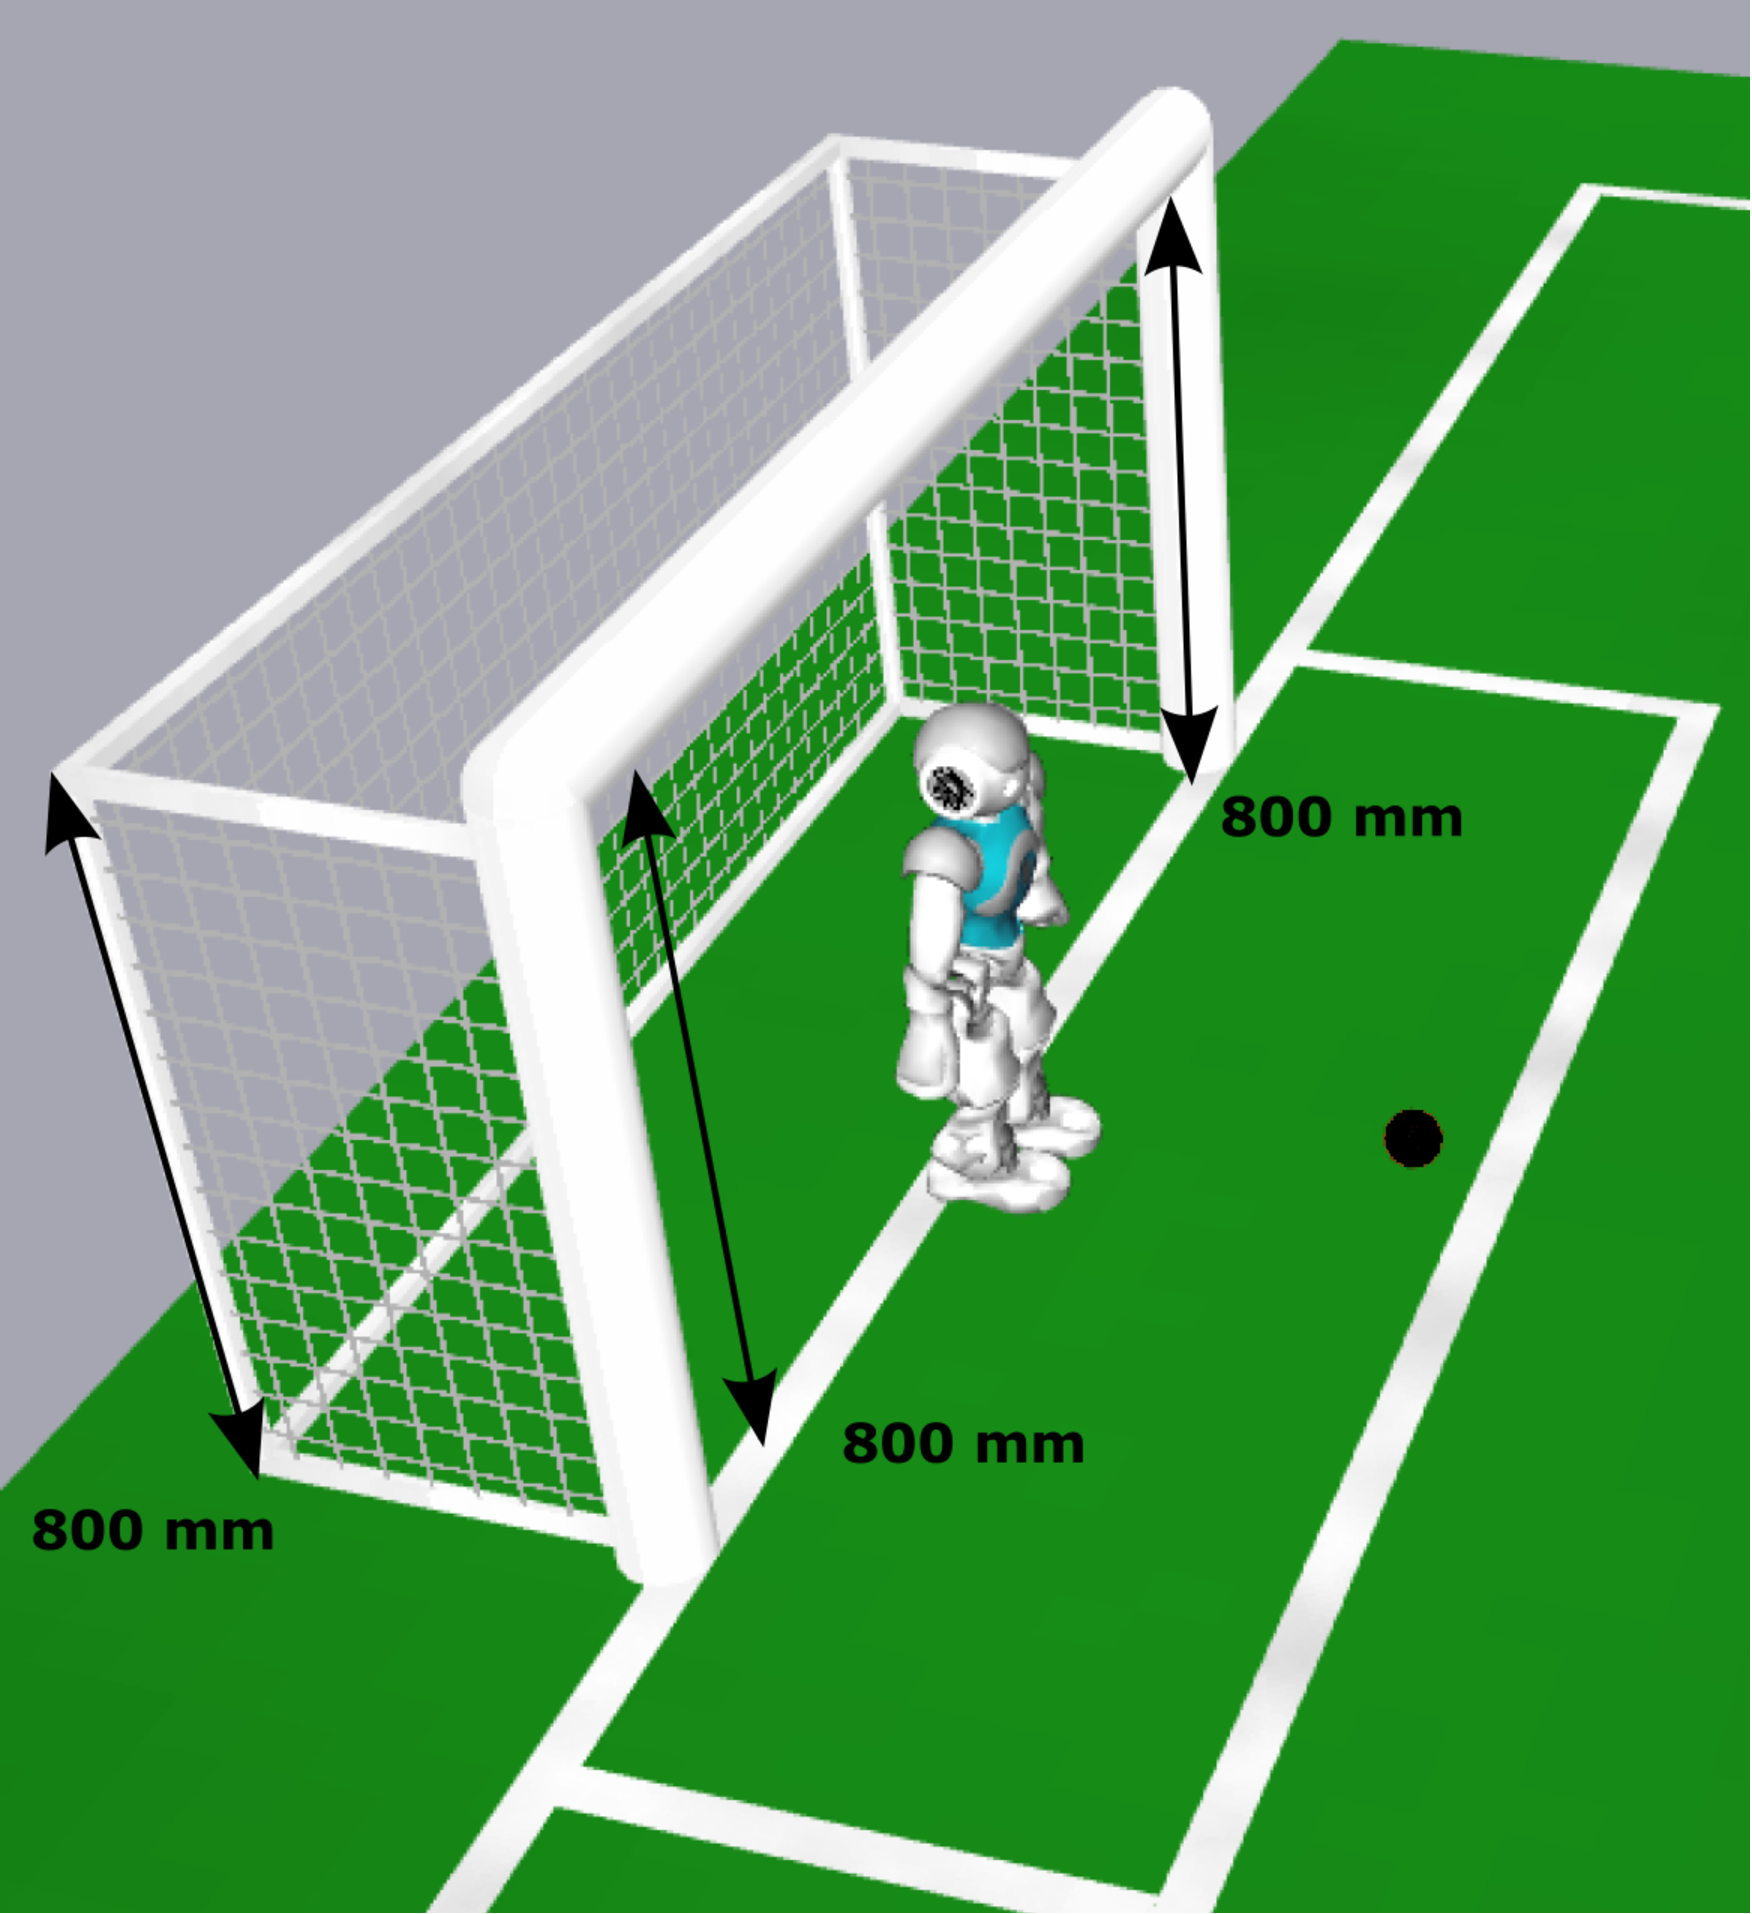
\includegraphics[width=1\columnwidth]{figs/goalDimensions3D.pdf}}%
		\end{minipage}
		\begin{minipage}[t]{0.49\columnwidth}
			The goalposts and crossbar are made from 3 white cylinders with a diameter of 100mm.
			The net:
			\begin{itemize}
				\item has a height of 800mm
				\item is of white, grey or black colour
				\item is tightly supported via the support structure, in a way to minimize interference with the goal keeper
				\item has a weave with holes smaller than the ball diameter.
			\end{itemize}
		\end{minipage}
		\caption{Appearance and dimensions of the goals.}
		\label{fig:goal_appearance}
	\end{center}
\end{figure}

\subsubsection{Field Colours}
\label{sec:field_colors}
The colours of the soccer field are as follow:

\begin{itemize}
	\item The field (artificial turf) itself is green (colour is not specified, but it should not be too dark).
	
	\item The lines on the field are white, whether they are taped, spray painted or made from white artificial turf.
	
	\item Goals~(\cf Figure~\ref{fig:goal_appearance}). The posts and top cross bar of both goals are white. The net and the support structure for the net are white, grey, or black.
\end{itemize}

\subsubsection{Lighting Conditions}
\label{sec:lightConditions}
The lighting conditions depend on the actual \cbw{game venue}. SPL fields \cbw{may} be placed near or under windows where possible. Whether or not window lighting is used, ceiling lights \cbw{should} be provided as necessary to ensure that most of the field is never darker than 300 Lux (400 Lux preferred).

\cbp{Nevertheless, it is not expected that teams should change the lighting setup in their local venue for the purpose of GORE 2021.} \\

Lighting is not required to be even and hotspots may occur on the field. The lighting design (comprising both natural and artificial light sources) shall aim to limit the ratio between the brightest and darkest patches on the field to less than 10:1. In general, lighting irregularities, including changes that occur during the competition, are acceptable and will not be cause for delay. Such irregularities may include sun streaming through windows, light bulbs turning off, light bulbs being replaced, etc.

\subsubsection{Ball}
\label{sec:ball}

The official ball is a soft foam ball with a black and white soccer ball print (see Figure~\ref{fig:ball}). They are 100mm in diameter and weigh 44 grams. These balls are available by writing to \url{info@sportpaint.de} (in German or English) and asking to order the "pu schaumstoffball 10cm 100ss".  Each ball costs EUR 2.50 plus shipping, where shipping cost depends on the destination.

\begin{figure}[t]
	\centerline{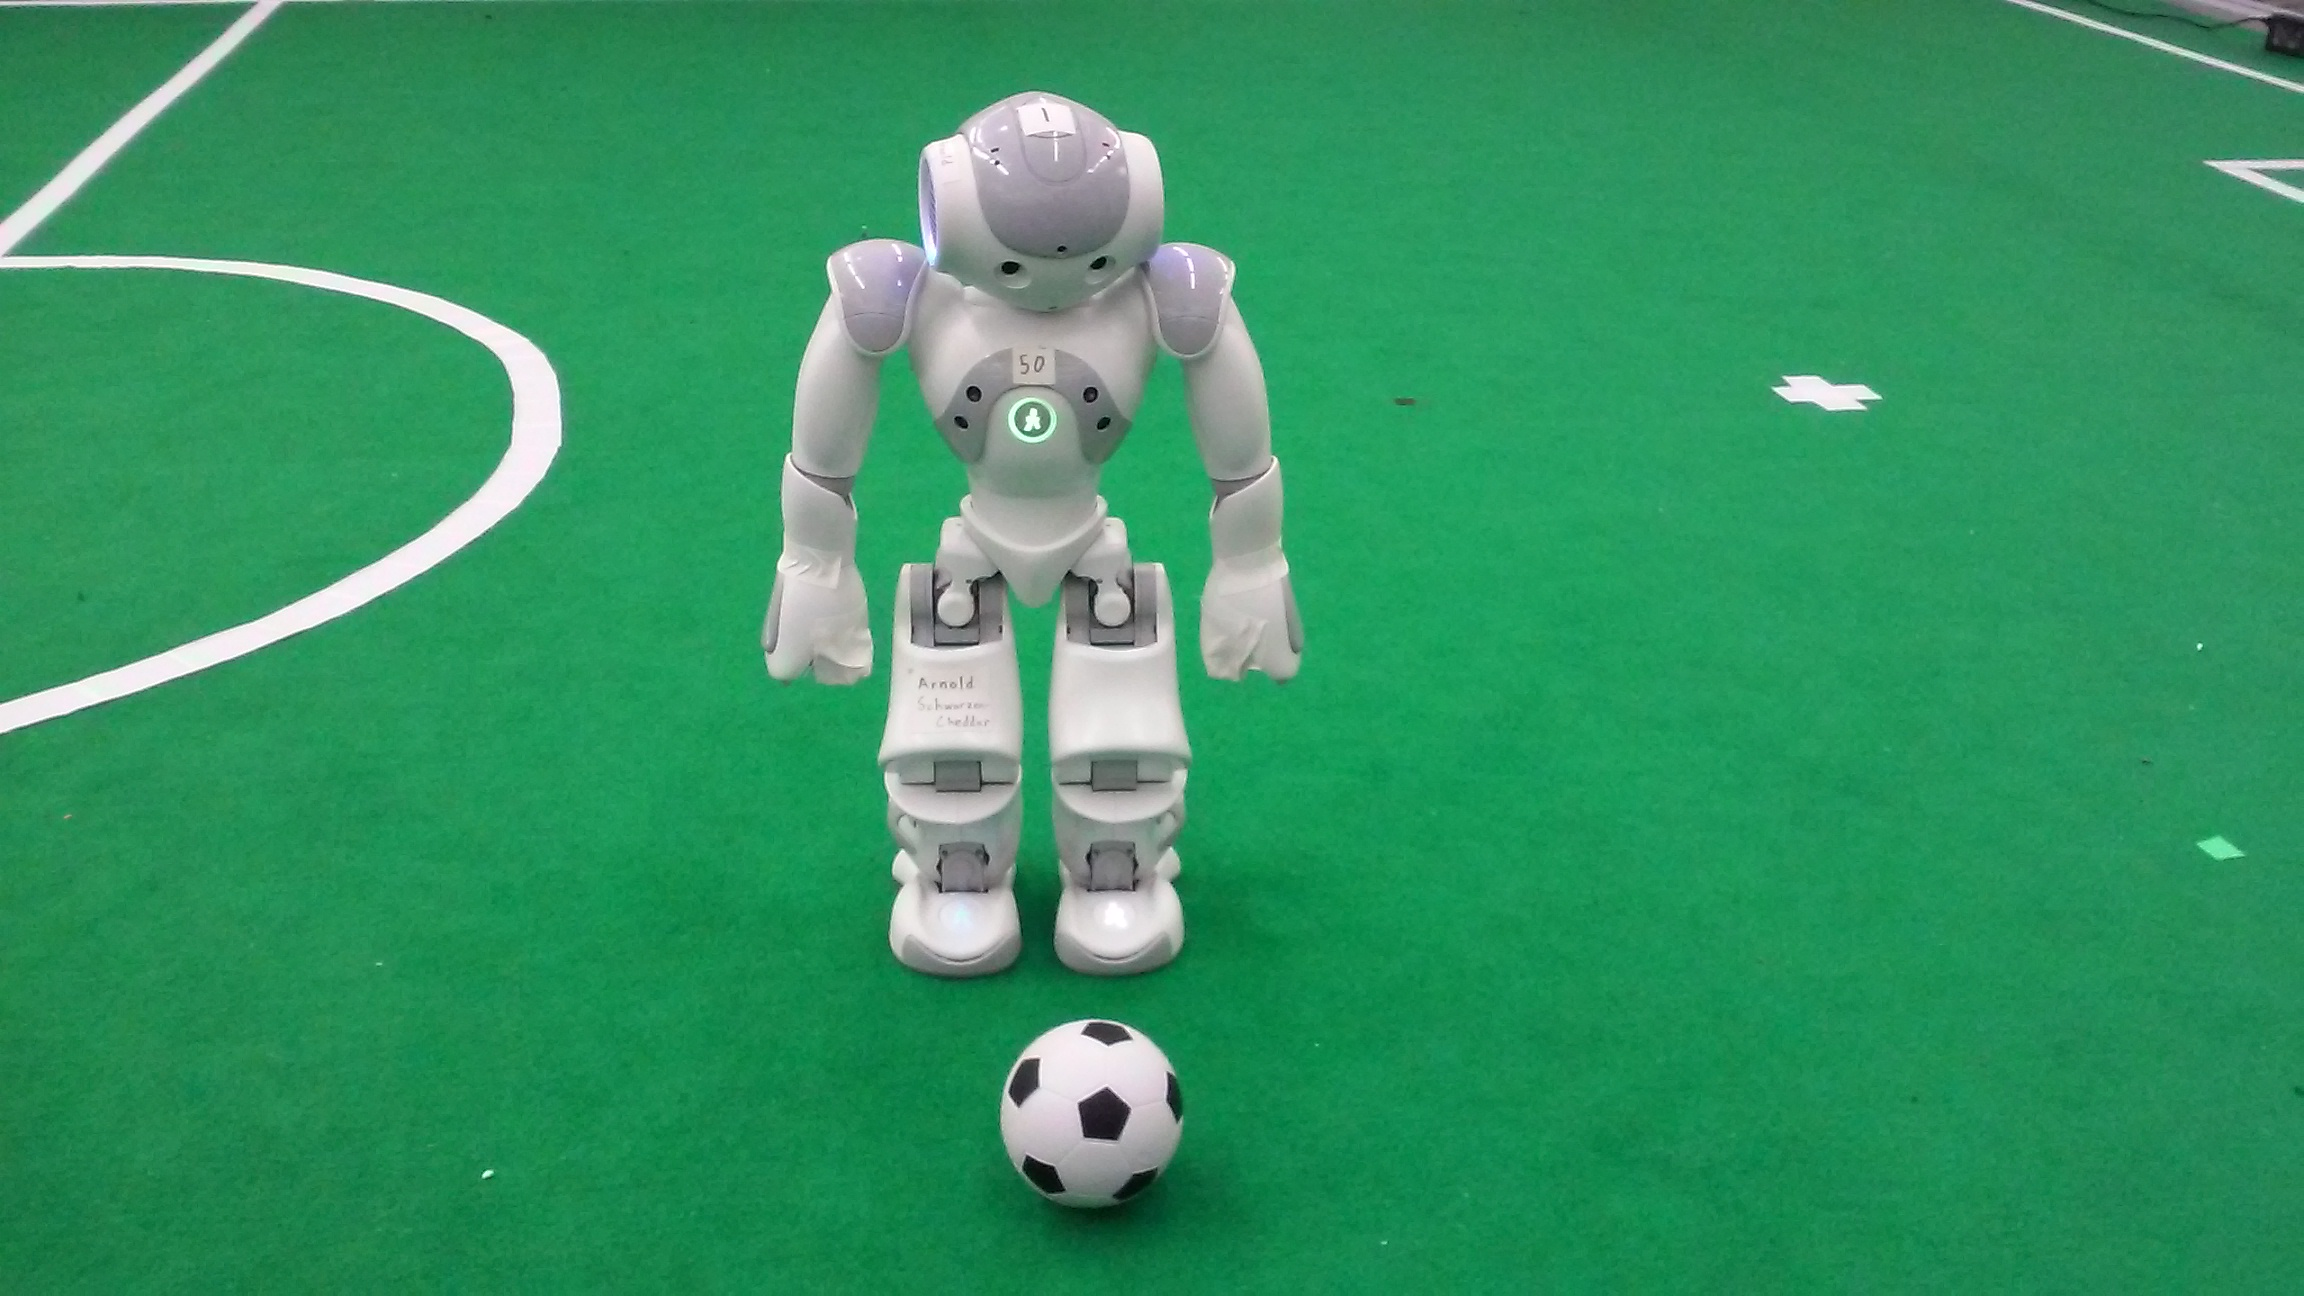
\includegraphics[height=0.28\columnwidth]{figs/robotWithBall2016.jpg}}
	\caption{A NAO and the official ball.}
	\label{fig:ball}
\end{figure}


\subsubsection{Definition of Inside and Outside}
\label{sec:inside_outside}

A line is always part of a region of the field.
This means, that \emph{inside/outside \textless region\textgreater} refers to the green area as well as the surrounding line.
Specifically:
\begin{itemize}
	\item The field boundary lines are part of the field
	\item The penalty box lines (and the end field line inside of the goal) are part of the penalty box
	\item The centre circle lines are part of the centre circle
\end{itemize}

The only \textit{exception} to this rule is the centre field line, which does not form part of any half.
That is, a robot is \textit{outside} of a half of the field if it is touching the centre line.

\cbp{\subsection{Streaming setup}
\label{sec:streaming_setup}

There are two use cases for the streaming setup: 
\begin{itemize}
	\item Allow participating teams to watch their games.
	\item Allow visitors to watch the games.
\end{itemize}

These cases should be taken into account when setting up a suitable streaming setup with respect to hardware equipment and internet connectivity.
You can think of streaming on YouTube/Discord/BigBlueButton/Zoom ..., whatever is available (If bandwidth in the lab is limited, re-streaming should be considered on system with better network connection).  
In the root folder of the NextCloud drive (see~\ref{sec:data_exchange}) you find a \texttt{streaming.md} file where every team has to publish a link that can be used by public and teams to watch the challenges. The public link will be published on the SPL website / RoboCup 2021 website.}


\subsection{Robot Players}
\label{sec:robot_players}
A match is played by two teams, each consisting of not more than \textbf{5} players. At most one player may be designated as \emph{goalkeeper}, the others are all \emph{field players}.

\subsubsection{Hardware}
\label{sec:hardware}
All teams must use a NAO humanoid robots \cbw{in version 6} manufactured by SoftBank Robotics.

Absolutely no modifications or additions to the robot hardware are allowed. No additional hardware is permitted including off-board sensing or processing systems. Additional sensors besides those originally installed on the robots are likewise not allowed. The only exceptions are:
\begin{itemize}
	\item Setting the passive wrist joints to a fixed position either with glue or a transparent or white duct tape.
	\item Protecting the fingers with white finger protectors provided by the manufacturer or with transparent or white duct tape.
	\item Placing white duct tape over the battery case and screw (under the robot jersey) to keep the battery case in place and prevent the battery becoming disconnected.
	\item A memory stick may remain in the head during operation.  Only ordinary USB flash memory keys that sit flush or recessed to the head casing may be utilized. Other USB dongles or devices, as well as memory sticks that are not flush or recessed, are not permitted.
\end{itemize}

A computer will be provided by the \cbw{host team} for the purpose of sending GameController messages to the robots.

\subsubsection{Goal Keeper}
\label{sec:goal_keeper}

The goal keeper is allowed to touch the ball with its arms/hands only while it is within its own \cbw{goal box area}. It always has the jersey number ``1''.

\subsubsection{Field Players}
\label{sec:field_players}
Each field player has a jersey number from the set $\{2, 3, 4, 5\}$. \\\cbw{There will be no 6th replacement robot}.

\subsubsection{Team Markers}
\label{sec:team_markers}
Robots use coloured jersey shirts as team markers in the ``home'' and ``away'' colours of the hosting arena team. Each jersey shirt has a player number (1-6) printed on it. The team markers are worn as shown in Figure~\ref{fig:nao_markers}.

\begin{figure}
	\centerline{\begin{tabular}{lll}
			a) & b) & c) \\
			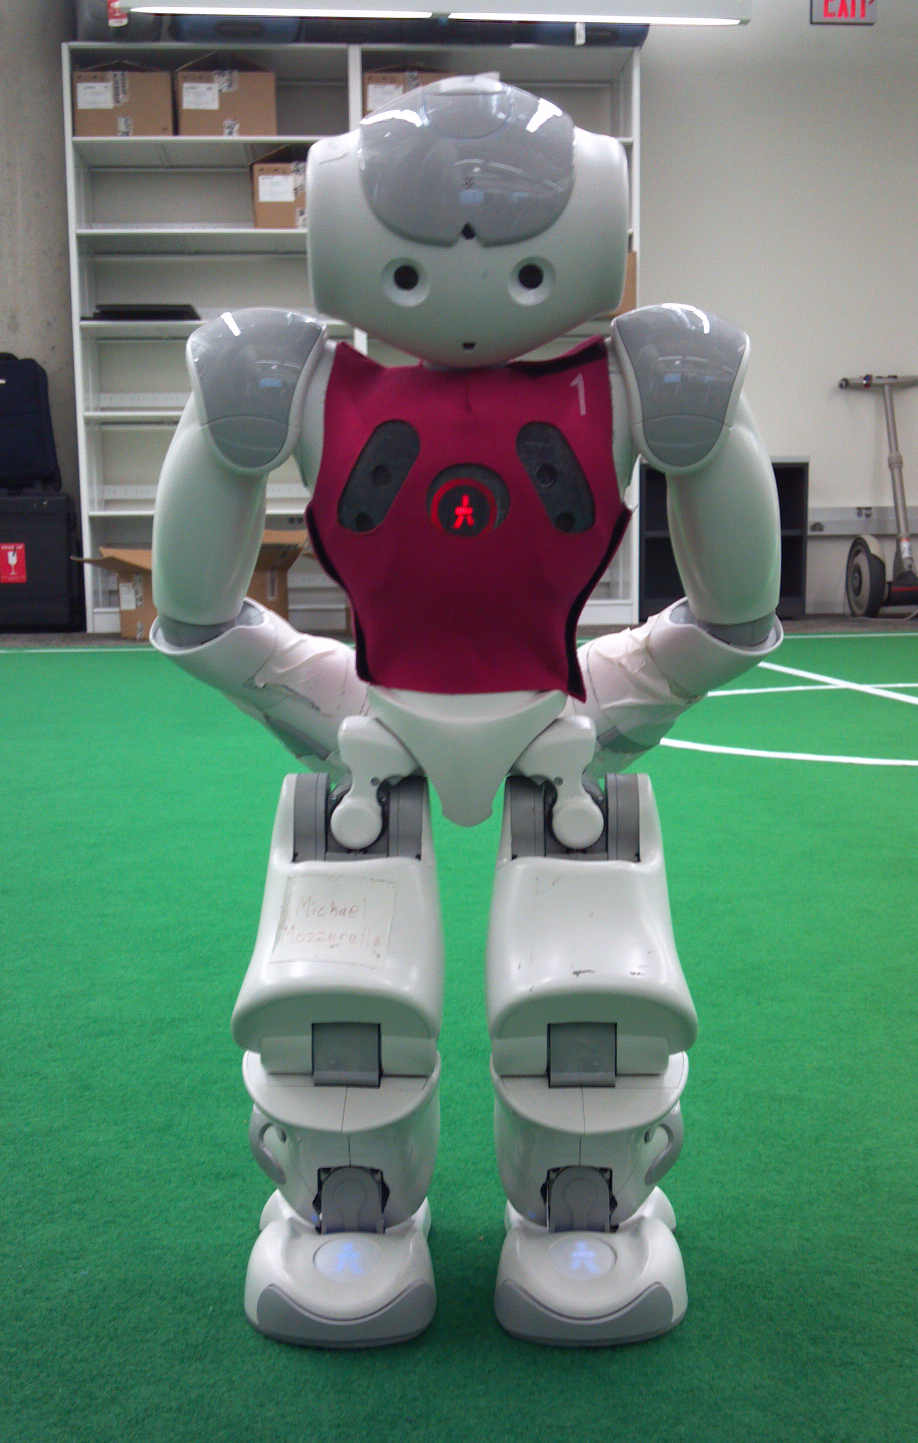
\includegraphics[height=0.28\columnwidth]{figs/front.jpg}&
			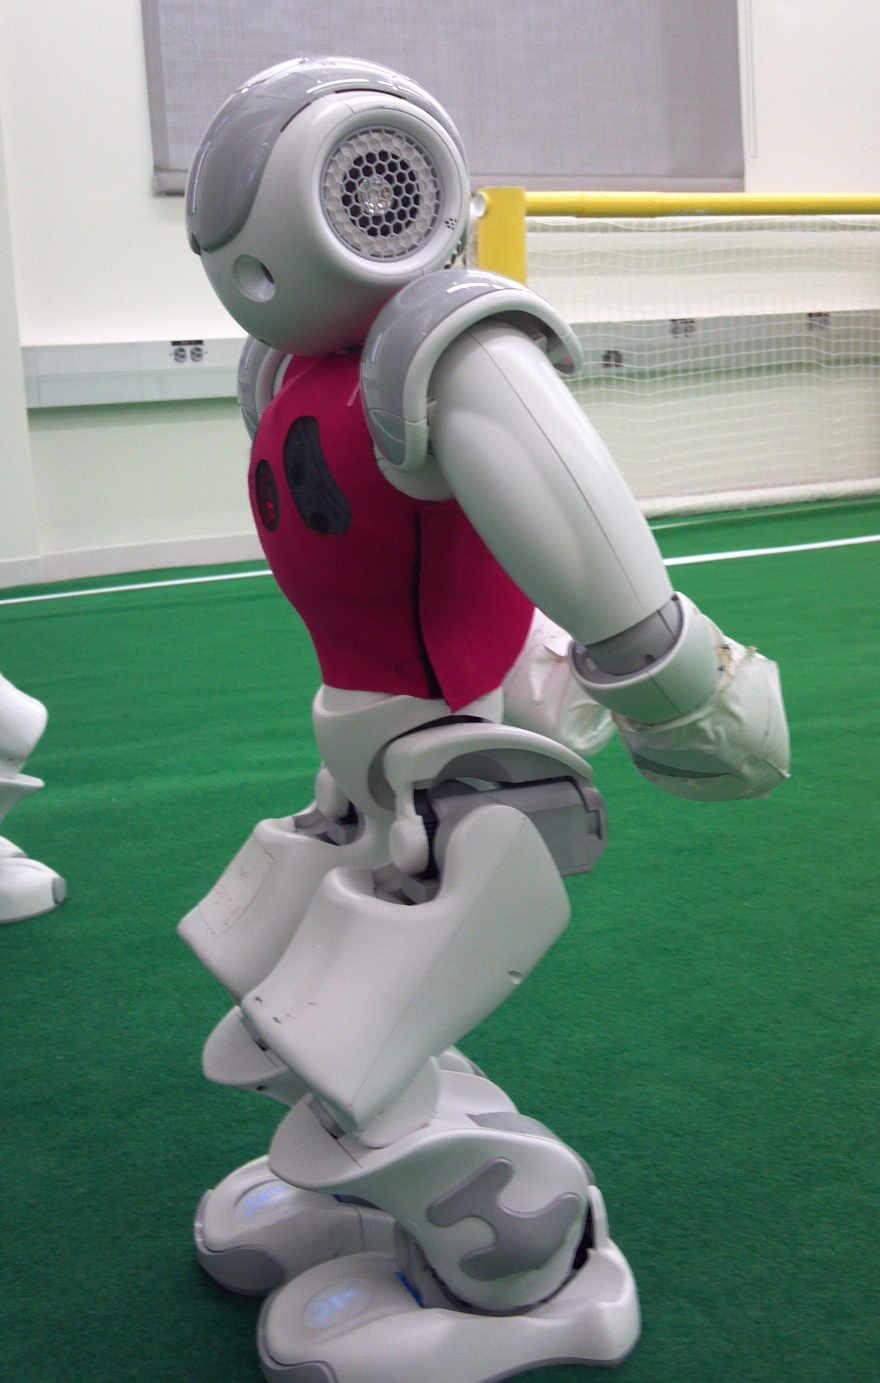
\includegraphics[height=0.28\columnwidth]{figs/side.jpg} &
			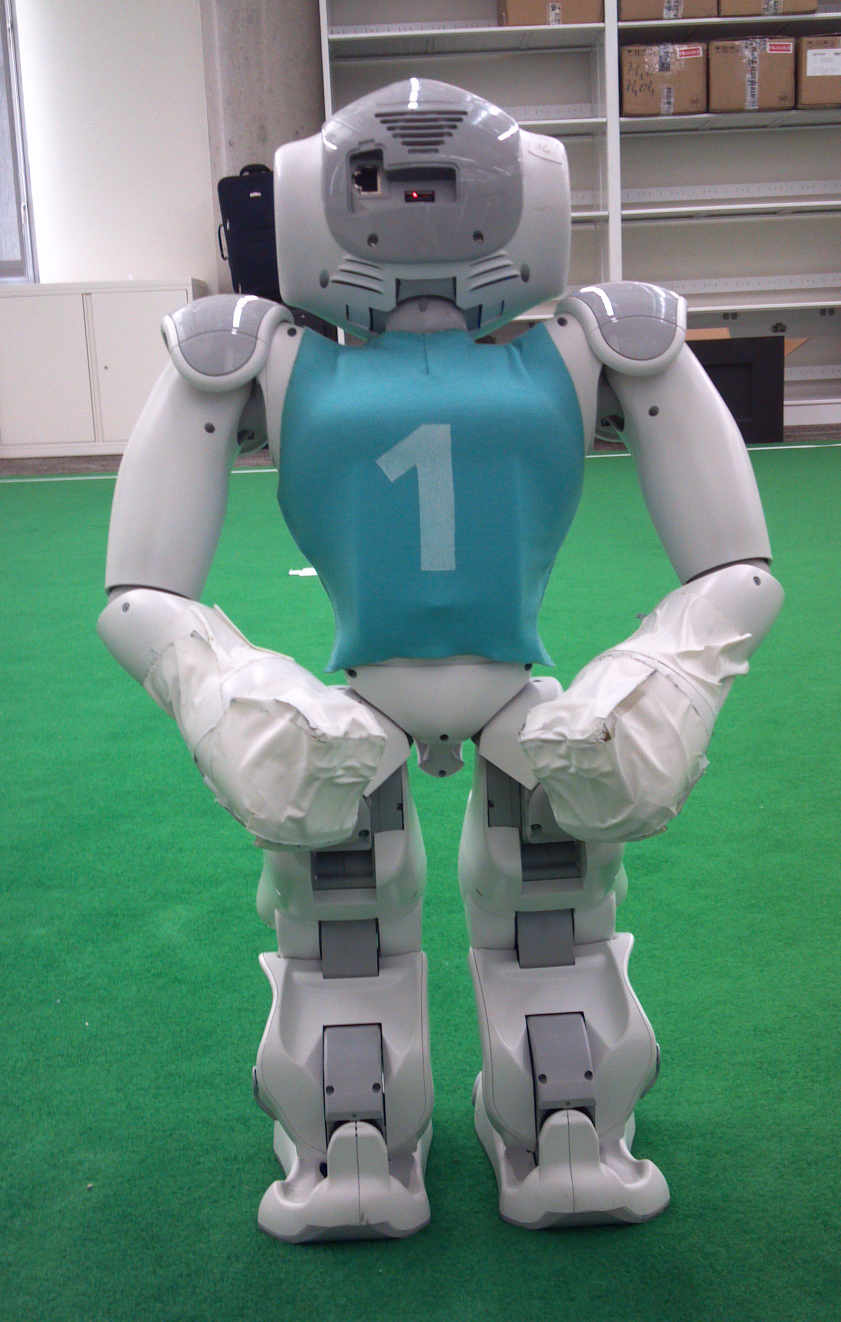
\includegraphics[height=0.28\columnwidth]{figs/back.jpg}
	\end{tabular} }
	\caption{Team markers. a) Front view. b) Side view. c) Back view.}
	\label{fig:nao_markers}
\end{figure}

\cbp{If a participating team wants to use their own jerseys (\eg because of sponsors logos) and has sent them to the hosting team all efforts should be made so that these jerseys can be used complying the followed guidelines.}

\cbp{Hosting teams/arenas must designate a ``home'' colour and an ``away'' colour when applying for GORE 2021. The team leaders can discuss the jersey assignment before the game. If no consensus is reached then the following applies:} 
Robots must wear the `home' jerseys when they are ``home'' (the first team listed on the schedule). The ``away'' team (the second team listed on the schedule) will wear the ``away'' jerseys.

\cbp{Teams may use any jersey that was approved for a RoboCup SPL competition in the last 4 years without needing to reapprove it in 2021.}

Teams may design and manufacture their own jerseys in any colour (multi and many colour jerseys are acceptable), but must follow these guidelines:
\begin{itemize}
	\item Jerseys should be the tank top style used at RoboCup 2013/2014 and should cover approximately the same areas of the robot as shown in Figure~\ref{fig:nao_markers}.  The torso LED must be clearly visible.  Jerseys may include the sonar panel used in the 2013/2014 jerseys, although this is not required.
	\item Jerseys must have a primary colour that comprises at least 70\% of the jersey.
	\item Jerseys should not contain distractors, such as large pictures of SPL balls or white stripes on green jerseys.
	\item All players on a team must wear identical jerseys.
	\item A team must wear the jerseys that it starts a game in for the entire game.
	\item Jersey material must be non-reflecting, non-shiny, and non-textured.  Material that is glittery is also not appropriate.
	\item Jerseys should be numbered 1-6 on both sides. The numbers must be large and {\bf easily} recognized by humans.
	\item \cbw{Hosting} teams must have two sets of jerseys that are significantly different in terms of their primary colour.
	\item Designs must be submitted to the GORE organizers for approval by May 1st, 2021. If the team has jersey prototypes, they should submit close-up images of a robot wearing the jersey - these images should be taken from front, back, and side angles. If the team has no prototypes, then designs depicting the expected jersey should be submitted. If submissions show separated front and back halves of jerseys then the team must specify which halves are matched to form home and away jerseys.  All images and designs should be submitted in pdf or jpg format.
\end{itemize}

Some teams wish to include additional information or logos on their robots. The following are allowable:
\begin{itemize}
	\item Attaching player numbers to the heads and/or legs of the robots.  These numbers should be black with a white background, and should correspond to the number on the robot's jersey.
	
	\item Adding sponsor or team logos to the upper legs of the robots (\cf Figure~\ref{fig:sponsor}). A box drawn around the non-white area of these logos must not cover more than a 25 $\text{cm}^2$ area. At most one logo may be attached per leg --- if you wish to attach more than one logo per leg, email the Technical Committee at least two weeks before the competition.  Depending on the size and design of the logos, this may be allowable.
	
	\item Adding small black and white stickers to the torso of the robots stating the name of the robot, the name of the team, or similar information. These stickers must be small and mostly white.
\end{itemize}

\begin{figure}[b]
	\centerline{\begin{tabular}{ll}
			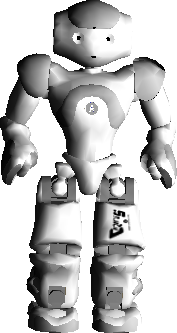
\includegraphics[height=0.35\columnwidth]{figs/naosim_with_logo.png}&
			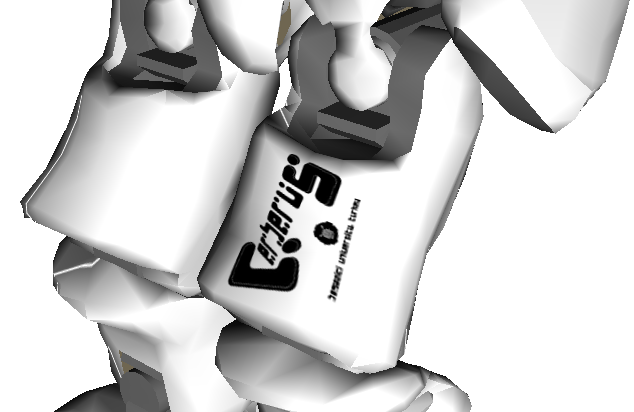
\includegraphics[height=0.35\columnwidth]{figs/naosim_legs_with_logo_closeup.png}
	\end{tabular}}
	\caption{Example Sponsor/Team Logo placement on legs.}
	\label{fig:sponsor}
\end{figure}

\subsubsection{Robot Pool Markers}
\label{sec:robot_pool_markers}
\cbp{In order to give each robot in the robot pool a unique ID (\cf Section~\ref{sec:robot_table}) that the hosting team can use to identify the robots, the hosting team is allowed to stick stickers/adhesive tape with the ID on it onto both upper arms of the robots and on the backside of the head.}

\subsubsection{Communications}
\label{sec:communications}
The robots must play without human control. Communication is only allowed among robots on the field and between the robots and the GameController.

\paragraph{Non-Wireless Communications}
\label{sec:acoustic}
In general there are no restrictions on communication between robots in play on the field using visual signalling (\eg gestures) or the robot's built-in microphones, speakers, and infrared transceivers. However, communication that causes excessive discomfort to an audience, affects the safety of an audience, or violates normal playing rules is not permitted.

\paragraph{Wireless Communications}
\label{sec:wireless}
The only wireless hardware allowed to be used by the teams/arenas are the wireless network cards built into the NAOs, and the access points provided by the arena. All other wireless hardware must be deactivated. A team/arena may be disqualified if one of the team members violates this rule.

Each team will get a range of IP addresses that can be used both for their robots and their computers/remote connections. The network configuration (\eg IP addresses, channels, SSIDs, and required encryption) of the fields \cbw{will be announced (\cf Section~\ref{sec:c3_BasicRequirementsForArenas})}.

Wireless robot-to-robot communication among the robot players is allowed, as long as it uses the access points provided by the event organizers (using the so-called ad-hoc mode is prohibited), messages are sent via UDP, the SPL standard message packet is used, and not more than one message per robot per second is sent\footnote{Official status packages that are sent to the GameController can be sent in addition to this message.}. The SPL standard message packet is specified in the header \emph{SPLStandardMessage.h} that is distributed with the latest GameController release. Each team will be assigned a range of IP-addresses that can be used for direct robot-to-robot communication. Each team will also be allocated a single UDP port on which broadcast will be permitted.  Specifically, a team's port will be 10000 plus that team's GameController number.

Teams and their robots must not listen into another team's communication.

Robots are not allowed to be connected to the access points \cbw{of the hosting arena if there} are currently running official games of other teams.

The GameController will use UDP to connect to the robots. The source distribution of the GameController provides the header file \emph{RoboCupGameControlData.h} that defines all messages sent by the GameController to the robots. They correspond to the \emph{robot states} described in Section~\ref{sec:robot_states}.

Robots send status updates (defined in \emph{RoboCupGameControlData.h}) to the GameController. These return packets must be addressed directly to the GameController PC (\ie not broadcast) and sent on the GameController return UDP port specified by the symbol \verb!GAMECONTROLLER_RETURN_PORT! in \emph{RoboCupGameControlData.h}.

The use of remote processing/sensing is prohibited.

\subsection{Game Process}
\label{sec:game_process}

\subsubsection{Structure of the Game}
\label{sec:game_struct}

A game consists of three parts, the first half, a half-time break, and the second half. Each half is 10 minutes counted from the initial kick-off.
The half-time break is ten minutes, and during this time both teams may \cbw{change robot programs}, or do anything else that can be done within the time allotted. \cbw{But there will be no replacement of robots!}

The head referee should make these whistle sounds from the T-junction of the half-way line \cbw{opposite from game controller}:
\begin{itemize}
\item The head referee signals the commencement of each half with a single whistle blow (that is, the Initial kick-off, \cf Section~\ref{sec:initial-kick-off}).
\item The head referee signals the end of the first half with two short whistle blows, and the end of the second half with two short plus one long whistle blow.
\end{itemize}

The teams/robots will change the goal defended during the half-time break.

\subsubsection{Robot States}
\label{sec:robot_states}

Robots can be in \textit{eight} different \emph{primary} states (\cf Figure~\ref{fig:robot_states}). \cbw{Wireless connection must be available}, so these states will be set by the GameController. Teams must implement code to receive and correctly respond to wireless GameController packets, and also give a visual indication of the game state.

\cbp{\textbf{The use of the button interface as a replacement for any GameController commands is not allowed in the GORE competition!}}

\cbp{Should, on both teams, at least \textbf{two} robots have problems with the Wifi/GameController connection the head referee should issue a referee timeout (\cf Section~\ref{sec:referee_timeout}).}
If \cbw{fewer} robots does not respond to the GameController then \cbw{they are, at the beginning,} not included in the game (via a `Request for Pick-up', \cbw{\cf Section~\ref{sec:request_for_pickup}}), and the game starts without the offending robots.

\begin{description}
    \item[Unstiff.] \cbw{\textit{This state has been added in 2021.}} It helps to facilitate a consistent and safe handling of the robots for remote competition. During any state, if all head buttons are pressed at least one second, the robot should move to a safe seated/crouched position and unstiffen all joints. Pressing the chest button once while in the \textit{unstiffen} state, permits the robot to stiffen it's joints and return to the initial state, or a state as indicated by GameController.

	\item[Initial.] After booting, the robots are in their \emph{initial} state. The robots are not allowed to be moving in any fashion besides initially standing up. Shortly pressing the chest button will switch the robot to the \emph{penalized} state.
	
	\item[Ready.] In this state, the robots walk to their legal positions for Kick-Off (\cf Section~\ref{sec:kick-off}) or a Penalty Kick (\cf Section~\ref{sec:penalty_free_kick})). They remain in this state, until the head referee decides that there is no significant progress, up to a maximum of \KickOffAutoTime.\\
    The GameController can activate substates for kick-off and penalty kicks.
	
	\item[Set.] In this state, the robots stop and wait for Kick-Off (\cf Section~\ref{sec:kick-off}).
	Illegally positioned robots are penalized \cbw{and placed on the side of the field.} Robots are allowed to move their heads or get up if fallen before the game (re)starts but they are not otherwise allowed to move their legs or locomote in any fashion. If a robot cannot get up, fallen robot is called (\cf Section~\ref{sec:fallenrobots}). The penalty time counter is frozen during this state.
	Note that all penalized robots are left in place (on the side of the field, or in-place for motion in set) and must wait to get unpenalized.\\
    The GameController can activate substates for kick-off and penalty kicks.
	
	\item[Playing.] In the \emph{playing} state, the robots are playing soccer. Shortly pressing the chest button will switch the robot to the \emph{penalized} state. During the \emph{playing} state, the GameController can activate the substates for free kicks (\cf Section~\ref{sec:free_kick}).
	
	\item[Penalized.] A robot is in this state when it has been penalized. It is not allowed to move in any fashion, this includes stopping the head turning. Shortly pressing the chest button will switch the robot back to the \emph{playing} state.
	
	\item[Finished.] This state is reached when a half is finished. \cbw{The robots then have to sit down.}

   	\item[Calibration.] \cbw{\textit{This state has been added in 2021.}} This state denotes the robot is acting with automatic calibration. This state may only be entered from Initial by pressing the \textit{front} head button plus the chest button.
    
\end{description}

\begin{figure}[t]
	\centerline{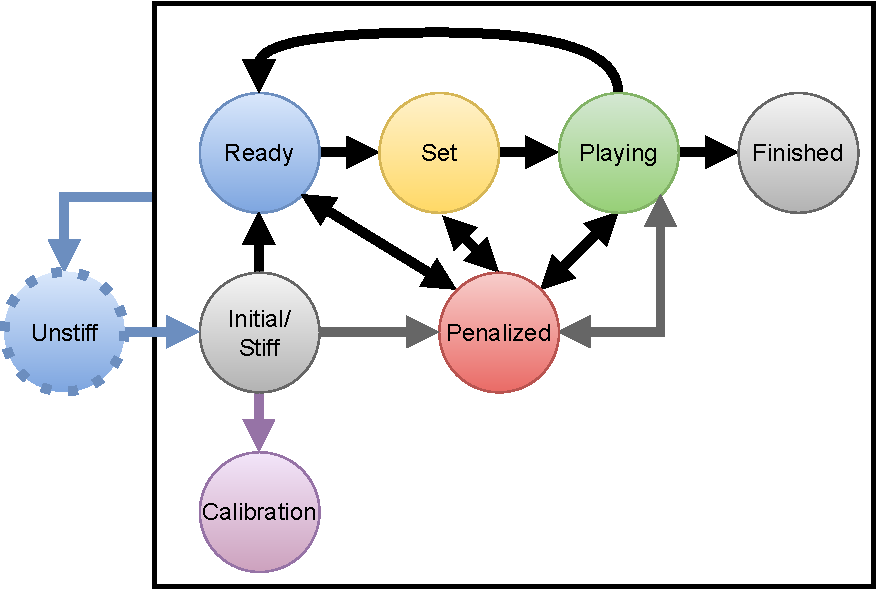
\includegraphics[width=0.9\columnwidth]{figs/states_new.pdf}}
	\caption{\cbf{Robot states with Unstiff as the start state. 
    \\\textbf{Chest button} transitions are shown as grey arrows. 
    \\\textbf{GameController} transitions are shown as black arrows. 
    \\\textbf{Calibration} transitions are shown as puple arrows which mean pressing the \textit{front head button plus the chest button}.
    \\ From \textbf{any state} it can be transitioned to the Unstiff state, as shown in blue arrows, via pressing all three head buttons at least one second.}}
	\label{fig:robot_states}
\end{figure}

The referee will announce the start of the \emph{playing} state with a single whistle blow.
The GameController \emph{playing} signal will be delayed by \PlayingDelayTime.
Robots that begin moving their legs or locomoting in any fashion during \emph{set} (\ie before the referee blows the whistle) will be penalized \textit{in place} on the field via the ``Motion in Set'' (\cf Section~\ref{sec:motion_in_set}) GameController signal (and moved back to their original position if they have moved significantly before becoming penalized) until the GameController transmits the \emph{playing} signal.

The current game state should be displayed on the LED in the torso. The colours corresponding to the game states are:

\begin{itemize}
    \item \cbw{Unstiff: Blue-Blinking}

	\item Initial: Off
	
	\item Ready: Blue
	
	\item Set: Yellow
	
	\item Playing: Green
	
	\item Penalized: Red
	
	\item Finished: Off

    \item \cbw{Calibration: Purple}
\end{itemize}

The current GameController requires robots to know both their team number and their robot number within the team. It is each team's responsibility to make sure this is correctly configured. It is recommended that the robot indicates its number within the team on boot-up so that this can be easily checked at the start of the game.

\subsubsection{Goal}
\label{sec:goal}
A goal \cbw{(including own goal)} is achieved when the entire ball (not only the centre of the ball) goes over the goal-side edge of the goal line, \ie the ball is completely inside the goal area\footnote{The goal line is part of the field.}. The restart after the goal shall adopt the same rules as the kick-off.

The head referee signals a goal by a single whistle blow, followed by the call ``Goal \textless colour\textgreater''. The head referee should point with one arm towards the center of the field.
To assist robots listening for whistles, the referee should blow the whistle from on the carpet at the end of the fields where the goal was scored.

The GameController signal (to the robots) of a goal being scored, will be delayed by \GoalScoredDelay.

\paragraph{Invalid Goal}
\label{sec:invalid_goal}
A goal is invalid (that is, it can never be awarded) in the following circumstances:
\begin{enumerate}
    \item When an Indirect Kick has not occurred (\cf Section~\ref{sec:indirect_kick}).
    \item When the last contact of the ball was with an attacking robot that played the ball with the arms/hands as defined in Section~\ref{sec:hand_ball}. However, an own goal may be scored by any defending robot playing with arms/hands.
    \item When a team scores on themselves (\ie own goal) and there are no opponent robots on the field that are active (a definition of \emph{active} is given in Section~\ref{sec:fallenrobots}).
\end{enumerate}

In these cases a goal is not scored (that is, the goal is ruled invalid) the game will proceed with a Goal Kick (\cf Section~\ref{sec:free_kick}). The head referee should also advice why the goal is invalid, such as by calling ``Not indirect''\cbw{, ``Played with hands'' or ``No own goal''.}

\paragraph{Indirect Kick}
\label{sec:indirect_kick}
From any restart in play (Kick-off, Kick-in, Free kick) except for Penalty kick, the attacking team may only score a goal via an indirect kick.

A robot may not score a goal from a direct kick, including via deflections.
The ball must be deliberately played-at a second time (by either another robot, or the same robot) before a goal may be scored.
A deliberate play at the ball includes successfully kicking the ball, dribbling the ball (and subsequently leaving possession of the ball), or the goalkeeper playing at the ball with its hands. 
\cbp{If a robot plays the ball to itself, this means that the ball must leave a circular area of at least \FreeKickRadius radius around the robot before the ball is played a second time and to be considered as an indirect kick.}

\textbf{Example 1:} Player 2 (of the red team) kicks the ball to Player 3, who then kicks the ball into the goal. This is a successful indirect kick, and the goal counts.

\textbf{Example 2:} Player 2 (of the red team), kicks the ball at the goal, and it is deflected of the side of the foot of a blue-team robot into the goal. This is \textit{not} an indirect kick, and the goal does not count.

\textbf{Example 3:} Player 2 (of the red team), kicks the ball ``upfield''. A blue-team robot kicks the ball a short distance, after which Player 2 kicks the ball again into the goal. This is a successful indirect kick, and the goal counts.

\textbf{Example 4:} Player 2 (of the red team), walks up to and dribbles the ball. To be an indirect kick, Player 2 must then stop, and visibly back-away from the ball, before approaching to dribble a \textit{second} time. The robot then scores. This is a successful indirect kick.

Note that an own-goal may always be scored without requiring an indirect kick.

\subsubsection{Initial Kick-off}
\label{sec:initial-kick-off}

The first kick-off at the start of each half is the initial kick-off.
Before the initial kick-off, \ie before the start of each half, all robots must be in the \cbw{\textit{unstiff} state} and will be placed on the sidelines, in their own half of the field, \cbw{by the referees acording to Figure~\ref{fig:initial_positions}}. 

\begin{figure}[t!]
	\begin{center}
		\leavevmode
		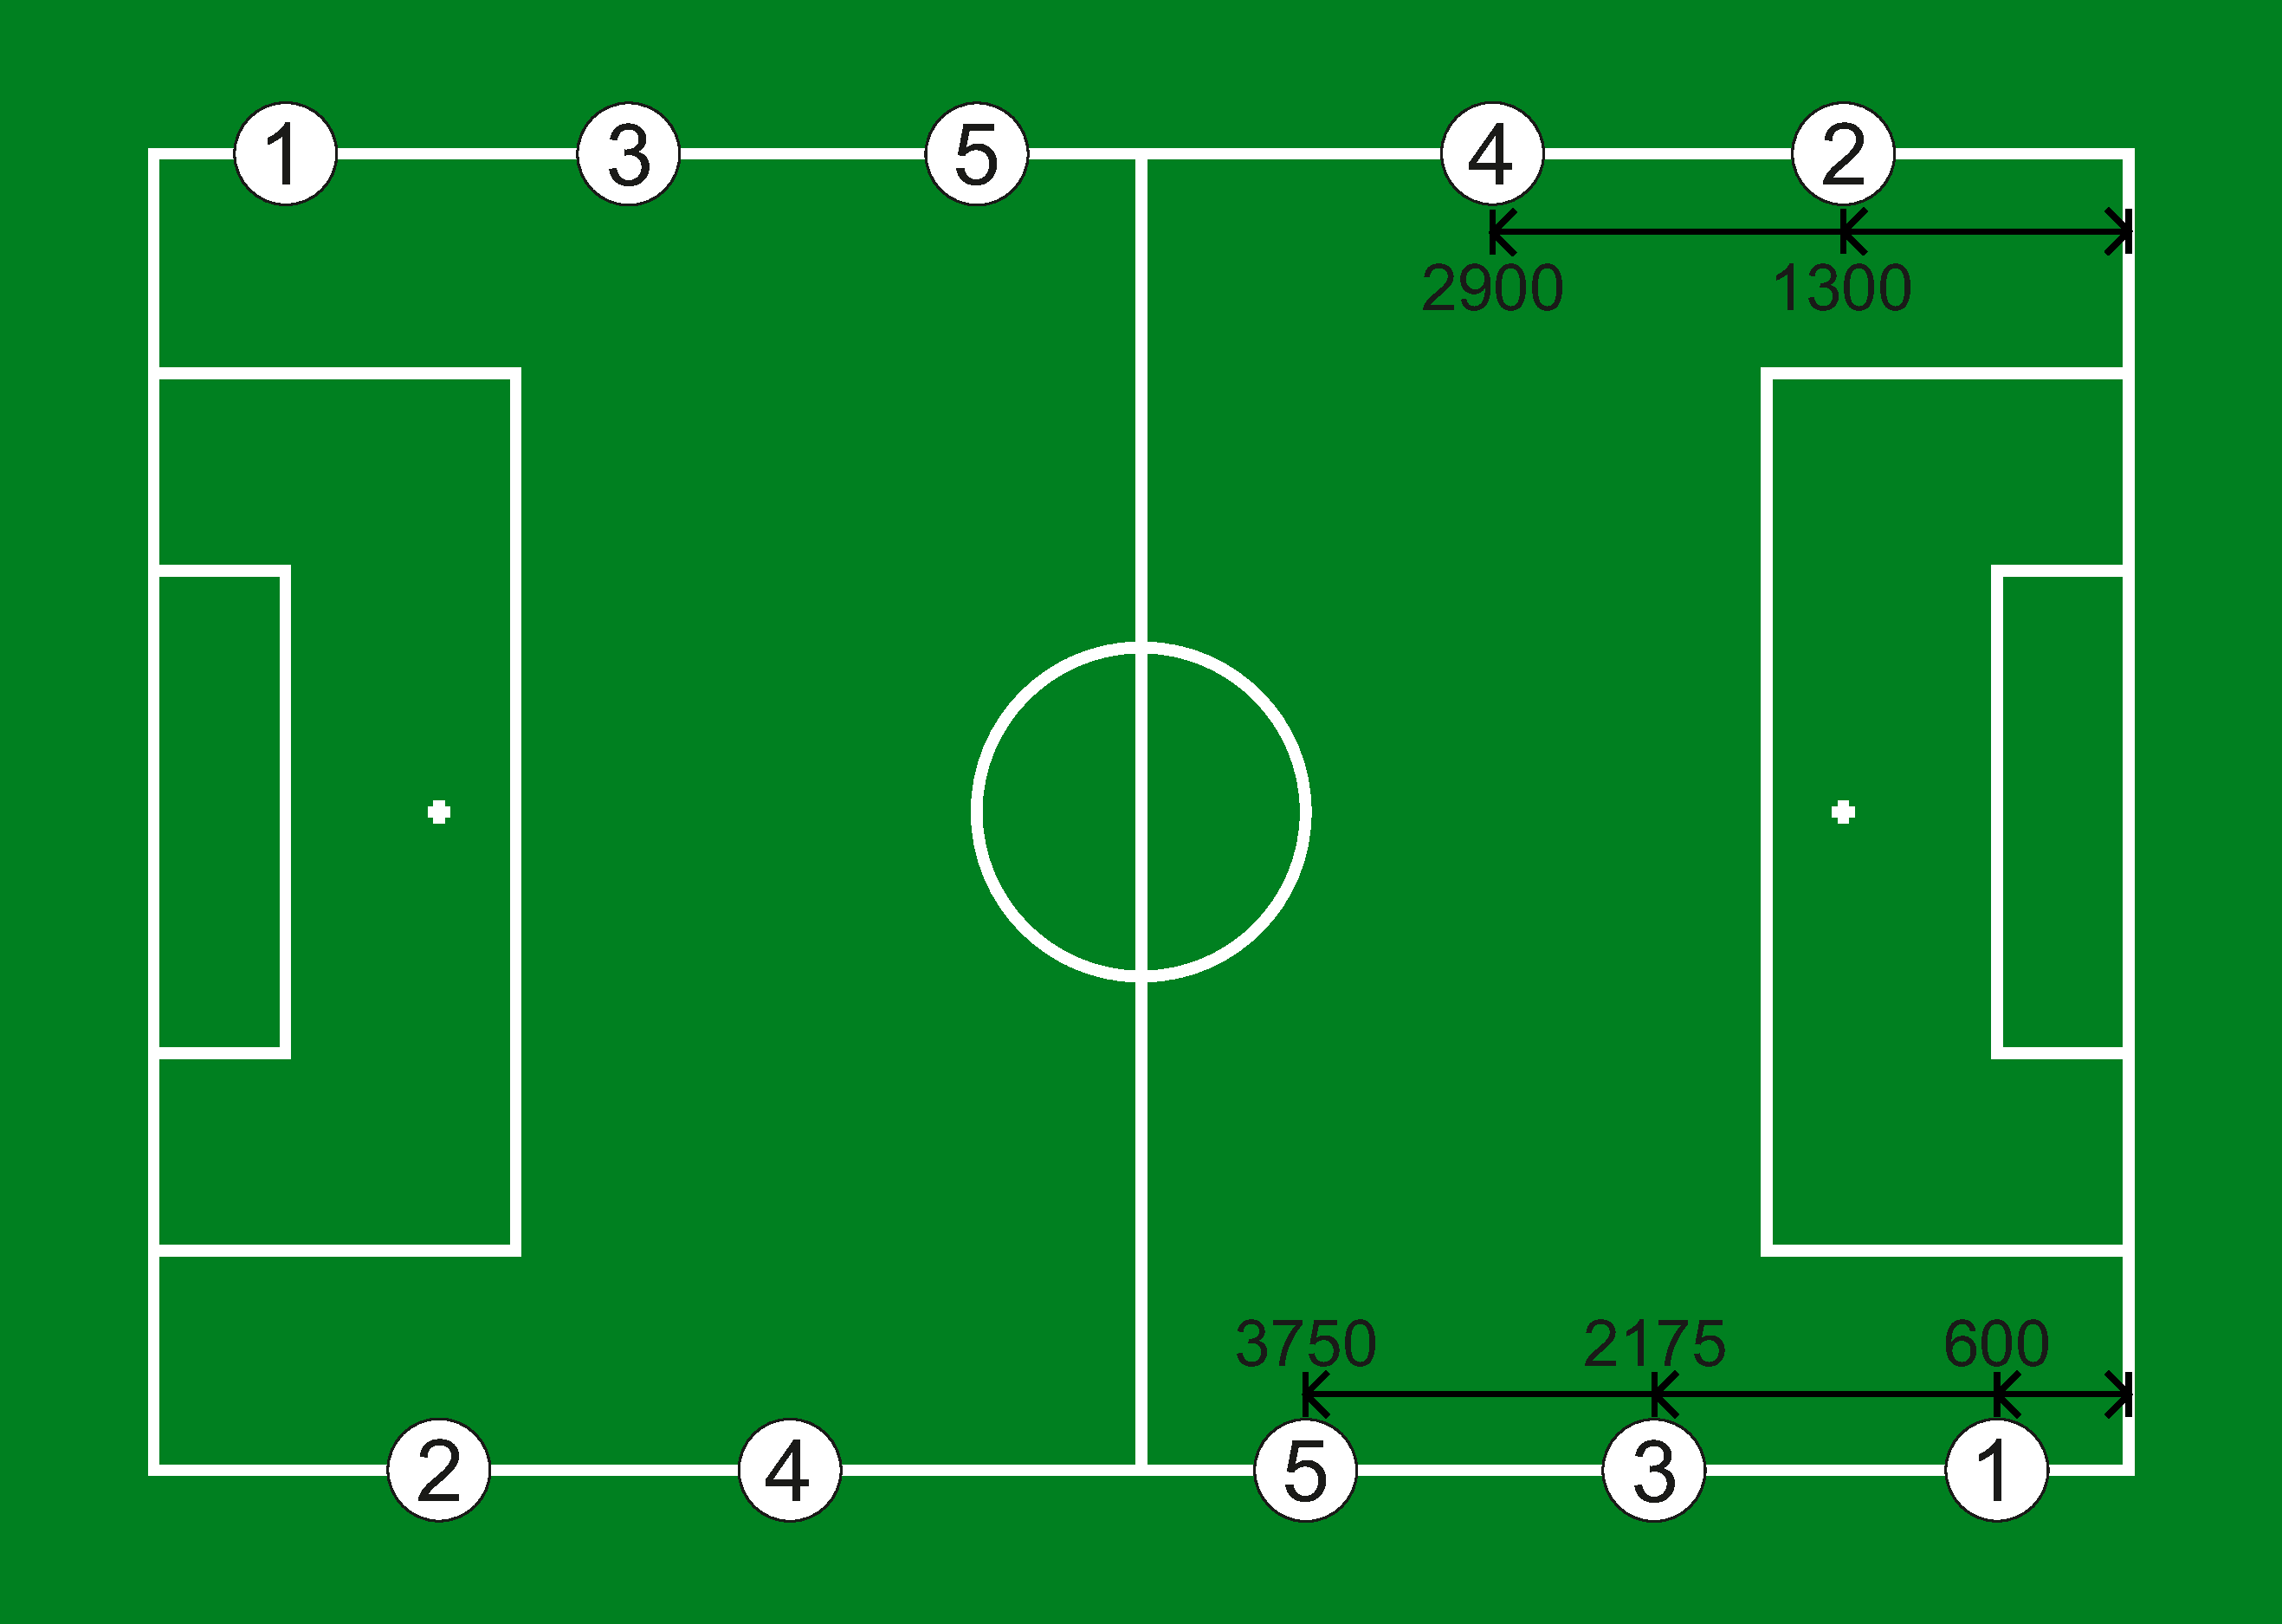
\includegraphics[width=1\columnwidth]{figs/initial_positions.pdf}
		\caption{Positions, player numbers and distances from the centre of the goal line for the initial kick-off of the robots.}
		\label{fig:initial_positions}
	\end{center}
\end{figure}


Once the robots receive the \emph{ready} signal from the GameController, they are to proceed as described in Section~\ref{sec:kick-off}.

\subsubsection{Kick-off}
\label{sec:kick-off}
For kick-off, the robots listening to the wireless GameController run through three states: \emph{ready}, \emph{set}, and \emph{playing}. \cbw{It is to a team's responsibility to have their robots listen to the GameController!}

In the ready state, the robots should walk to their legal kick-off positions.
The attacking team can be positioned anywhere within their own half.
The defending team can be positioned within their own half, except for inside the center circle.
No player is allowed to touch the halfway line.
Both teams are also subject to restrictions on the penalty box~(\cf Section~\ref{sec:illegal_positioning}).
The green carpet border, except for the area of the goal, is not part of either teams own half. All robots that do not reach legal positions will be penalized with the ``Illegal Position'' penalty~(\cf Section~\ref{sec:illegal_positioning}).

In the \emph{set} state, the robots must not locomote~(\cf Section~\ref{sec:robot_states}). A referee places the ball on the center point of the center circle. If the ball is moved by one of the robots during \emph{set} it is replaced by one of the referees.

\cbp{There is no manual placement of any robot.}

The head referee signals the kick-off by a single whistle blow, followed by the call ``Playing''. The head referee must signal this from the T-junction of the half-way line.

After the head referee has signalled the kick-off, the robot's state is switched to \emph{playing} \cbw{by the GameController}.
The defensive team must stay outside of the center circle until the ball is in play. The ball is in play once it is touched by the attacking team or once \emph{\KickOffBallFreeTime} have elapsed in the playing state. The GameController and head referee will indicate this by the call `` Ball Free''. If a defensive player enters the center circle before the ball is in play, the ``Illegal Position'' penalty is applied (\cf Section~\ref{sec:illegal_positioning}).

Note a goal may not be scored from within the center circle on kick-off~(\cf Section~\ref{sec:invalid_goal}), and that indirect kick rules apply~(\cf Section~\ref{sec:indirect_kick}).

\subsubsection{Kick-in}
\label{sec:kick_in}
A ball is considered to have left the field when there is no part of the ball over the outside of the boundary line (\ie the line itself is in). If the ball leaves the field it will be replaced on the field by an assistant referee. Balls are deemed to be out based on the team that last touched the ball, irrespective of who actually kicked the ball.

If the ball goes over a sideline then the assistant referee will replace the ball back on the point of that sideline where it went out. A free kick (\cf Section~\ref{sec:free_kick}) is awarded to the team that did \emph{not} last touch the ball by the referee calling ``Kick-in \textless color\textgreater''.

If the ball goes over an end-line then the assistant referee will replace the ball back on the field, depending on which team last touched the ball:
\begin{itemize}
\item If the ball was last touched by the \textbf{defensive} team, a \emph{Corner Kick} (\cf Section~\ref{sec:free_kick}) is awarded to the attacking team. The referee calls ``Corner Kick \textless colour\textgreater'' and the ball is placed on the corner on the same side of the field that the ball was kicked-out.
\item If the ball was last touched by the \textbf{offensive} team, a \emph{Goal Kick} (\cf Section~\ref{sec:free_kick}) is awarded to the defensive team. The referee calls ``Goal Kick \textless colour\textgreater'', and the ball is placed on the corner of the goalbox on the same side of the field that the ball was kicked-out. That is, the corner inside the field, not the t-junction where the goalbox meets the goal line.
\end{itemize}

\paragraph{Example 1.} The red goal keeper kicks the ball out the end of the field to the right of the goal. The referee calls ``Corner Kick blue'', the ball is placed on the corner to the right of the goal and a free kick is started.

\paragraph{Example 2.} A blue robot kicks the ball out the end of the field to the right of the goal the red team is defending. The referee calls ``Goal Kick red'' and the ball is placed on the right corner of the goalbox.

\paragraph{Example 3.} A blue robot at midfield kicks the ball over the left sideline 2 meters into the half of the field the red team is defending. The referee calls ``Kick-in red'' and the ball is replaced on the left sideline where it went out.

\paragraph{Example 4.} A blue robot kicks the ball but the ball touches a red robot at midfield before leaving the field near the center line. The ball is regarded as out by red, the referee calls ``Kick-in blue'' and the ball is replaced on the kick-in line where it went out.

\subsubsection{Free Kick}
\label{sec:free_kick}
A Free Kick is initiated:
\begin{itemize}
  \item When the ball goes over the sidelines, termed \textbf{Kick-in}.
  \item When the ball goes over the end-lines initiated by the defensive team, termed \textbf{Corner Kick}.
  \item Instead of an end-line Kick-in initiated by the offensive team, also termed a \textbf{Goal Kick}.
  \item A pushing penalty (see Section~\ref{sec:player_pushing}) awarded near the ball, termed a \textbf{Pushing Free Kick}.
  \item A pushing penalty (see Section~\ref{sec:player_pushing}) awarded against the defending team within their own penalty box, termed a \textbf{Penalty Kick}.
\end{itemize}

The head referee will announce a Free Kick, calling one of:
\begin{enumerate}
  \item For a \textbf{Pushing Free Kick}: ``Foul \textless color\textgreater \textless number\textgreater'' for the pushing robot.
  \item For a \textbf{Penalty Kick}: ``Foul \textless color\textgreater \textless number\textgreater'' for the pushing robot, followed by ``Penalty Kick \textless team\textgreater''.
  \item For all \textbf{other free kicks}: ``Kick-in/Goal Kick/Corner Kick \textless team\textgreater'' for the team that did not last touch the ball.
\end{enumerate}

The GameController will then activate the substate for the respective free kick. Note that in the case of the Pushing Free Kick the substate is activated automatically through the ``Foul''. The team who is awarded the Free Kick (termed the attacking team) has \FreeKickTime to complete the kick. For a ``Penalty Kick'', the game instead proceeds as described in Section~\ref{sec:penalty_free_kick}.

When necessary, the referee may need to place the ball. For a Pushing Free Kick, the ball will be left in place, and only repositioned in accordance with the pushing rules (see Section~\ref{sec:player_pushing}). If the ball left the field, the ball will be positioned as described in Section~\ref{sec:kick_in}.

During the Free Kick, only the attacking team may approach within \FreeKickRadius to the ball, with the exception of the defensive goalkeeper. All other robots of the defensive team must move away from the ball. The defensive goalkeeper may be within the \FreeKickRadius radius, provided that it is within the Penalty Box and does not touch the ball.\\
Defensive robots that violate these restrictions are penalised with the ``Illegal Positioning'' penalty (see Section~\ref{sec:illegal_positioning}) which results in a standard removal penalty~(see Section~\ref{sec:removal_penalty}).

Additional penalties against any further robots during the free kick, including Pushing, do not result in an additional Free Kick, but still use the appropriate removal penalty.

A Free Kick is deemed completed and play returns to normal if:
\begin{itemize}
    \item The attacking team touches the ball, except for a robot getting up which is exempt from this rule.
    \item The \FreeKickTime time period expires (or the game time expires).
\end{itemize}
The head referee will announce a Free Kick is completed, by ``Ball Free'', and the GameController resumes the game state \emph{playing}. Note that the substate will be automatically left after the \FreeKickTime time period expires.

\paragraph{Penalty Kick Procedure}
\label{sec:penalty_free_kick}

When the GameController activates the Penalty Kick, the game changes to the \textit{ready} state. This denotes that the robot's are given time to setup and prepare for the penalty kick. Similar to kick-off, the game clock is \textit{paused} during finals games only. The referees should pick up the ball.

Robots have \PenaltyFreeKickSetupTime to get into position for the Penalty Kick. At the end of 30 seconds, the game changes to the \textit{set} state. Similar to a kick-off, during the \textit{set} state the robots are waiting for the Penalty Kick to commence. Standard penalties apply. \\
Additionally, only the goalkeeper robot from the defending team may be within the penalty box. The goalkeeper robot must also be touching the goal line. Only one robot from the attacking team may be within the penalty box, and it may not block the penalty spot. Blocking the penalty spot is considered to be an illegal position. All robots that do not reach legal positions will be penalized with the ``Illegal Positioning'' penalty~(\cf Section~\ref{sec:illegal_positioning}).

During \textit{set} the referee should place the ball on the penalty spot and afterwards the referee signals the Penalty Kick commences by blowing the whistle once, and calling ``Playing''. The game switches to the \textit{free kick} sub-state of the \textit{playing} game state, and the game clock is resumed. (Note that the GameContoller signal is delayed by \PlayingDelayTime when switching from \textit{set} to \textit{free kick} sub-state). The attacking team has \PenaltyFreeKickTime to complete the Penalty Kick.

During the Penalty Kick:
\begin{enumerate}
    \item The defensive goalkeeper robot must always be in contact with the goal line, and must remain on its feet. The goalkeeper is only permitted to ``dive'', and be off it's feet after the attacking robot has touched the ball.
    \item The attacking robot may move freely.
    \item All robots must be within the field-of-play. That is, robots may not be outside the field lines, but within the field border.
    \item No other robots may enter the penalty box (\cf Section~\ref{sec:illegal_positioning}).
    \item Additional penalties against any further robots, including Pushing, do not result in an additional Free
    Kick, but still use the appropriate removal penalty.
\end{enumerate}

The attacking robot (taking the penalty kick) may only score a goal if it touches the ball once. Once the attacking robot has touched the ball, it may not score a goal until another robot (from either team) touches the ball. If, in this case, the robot ``scores'' it results in a ``Goal Kick""~(\cf Section~\ref{sec:invalid_goal}).

The Penalty Kick is deemed completed if:
\begin{itemize}
\item The attacking team touches the ball, even if the robot has fallen.
\item The \PenaltyFreeKickTime time period expires (or the game time expires).
\end{itemize}

The head referee will announce a Free Kick is completed, by ``Ball Free'', and the GameController resumes the game state \emph{playing}. Note that the substate will be automatically left (returning to the \textit{playing} state) after the \PenaltyFreeKickTime time period expires.

Note that the restrictions on the attacking robot still apply after the penalty kick is complete.

\subsubsection{Game Stuck}
\label{sec:game_stuck}

In the event of no substantial change in the game state for 30 seconds, this is considered a game stuck. ``Substantial change'' can consist of a robot seeing and moving towards the ball OR robots exploring the field (presumably in an attempt to find the ball).

The main referee has two options how to solve the game stuck and to reestablish the chance of progress in the game. The intention of the game stuck rule is to achieve progress with as little intervention as possible, \ie the \emph{Local Game Stuck} rule will be preferred, but only if there is a chance that its application will result in progress in the game.

\paragraph{Local Game Stuck}
\label{sec:game_stuck:local}

If one robot is preventing the game from proceeding --- perhaps by circling the ball repeatedly without kicking the ball --- it is recommended to improve progress by removing this one robot.
The head referee calls ``Local Game Stuck \textless robot\textgreater'' for this robot, which is penalised (\cf Section~\ref{sec:pen_local_game_stuck}).

\paragraph{Global Game Stuck}
\label{sec:game_stuck:global}

If no robots have made progress towards the ball or began to explore the field in 30 seconds, Global Game Stuck should be called on the team whose robot is \textit{not} nearest the ball.
The referee calls ``Global Game Stuck \textless colour\textgreater''.

Once the referee calls Global Game Stuck, players enter the Ready state, and a new kick-off is awarded to the team that was closer to the ball when the Global Game Stuck was called. A global game stuck can only be called if at least one robot has touched the ball since the previous kick-off.

\subsubsection{Request for Pick-up}
\label{sec:request_for_pickup}

Either team may request that their players be picked up (called ``Request for Pick-up''). In the Playing or Ready state, players may only be picked up for hardware failures. In all other states, players may be picked up for any reason.

Every change (hardware or software) is allowed during a request for pick-up. In particular, it is permitted to change batteries, fix mechanical problems, reboot the robots, and change configuration files. It is discouraged to change the robot's control program, \textbf{but not forbidden}. \\
\cbp{Since the teams are not on site, the assistant referees take over these tasks as if they were a member of the corresponding team.}

Any strategic ``Request for Pick-up'' is not allowed. That is, gaining an advantage by removing the robot from the competition. In this case, the head referee will indicate when the robot is no longer affecting play and can be removed from the field by an assistant referee.

To prevent mistakes and confusion during games, only team leaders should make a ``Request for Pick-up''. \change{Referenz zu eigenem Discord channel mit einem der Assistants?}

The returning robot may be returned following the normal replacement procedure once at least 45 seconds have elapsed since the robot was removed from play. Note that this penalty does not follow the standard removal procedure, and hence does not count towards the incremental penalty count.

If the picked-up robot was penalized, the penalty time of the robot counts down with the game clock throughout the pick-up.
Note here, that the returning robot will have to wait out any remaining penalty time of the picked up robot after \cbw{the robots are ready again}.

\subsubsection{Request for Timeout}
\label{sec:request_for_timeout}
Each team can call a \textbf{maximum of 1 timeout per game} with a total time of no more than \textbf{5 minutes}. During this time, both teams may \cbw{change robot programs}, or do anything else that can be done within the time allotted. \cbw{But there will be no replacement of robots!}\\
\cbp{Since the teams are not on site, the assistant referees take over these tasks as if they were a member of the corresponding team.}

During normal game time, a team may call a timeout at any stoppage of play (after a goal, stuck game, before a half, etc.). Alternatively, a team may call a timeout before a penalty shootout if they have not used their timeout yet (\cf Section~\ref{sec:penalty_shoot-out}).

The timeout ends when the team that called the timeout says they are finished, at which time they must be ready to play. The other team must be ready to play at the time the timeout runs out, or \textbf{2 minutes} after a prematurely called end of the timeout, whichever is earlier. If the other team is not ready to play in time, it has to call a timeout of its own.

The clock stops during timeouts, even during the preliminaries, and is reset to the time when the current stoppage of play began.

After the completion of the timeout, the game resumes with a kick off for the team which did not call the timeout.

If a team is not ready to play at the assigned time for a game, the referee will call the timeout for that team. After the expiration of such a timeout, if the team is still not ready to play then the referee shall start the game with only one team on the field.  The team that was not ready can return its robots to the field as per the rules for ``Request for Pick-up''. 

If both teams are not ready, the referee will call timeouts for both teams. This ``double timeout'' expires after 5 + 5 = 10 minutes.

\subsubsection{Referee Timeout}
\label{sec:referee_timeout}
The head official may call a timeout at any stoppage of play if he or she deems it necessary. A referee timeout should only be called in dire circumstances --- one example might be when the power to the wireless router is down \cbw{or no robot listens to the GameController}. However, when and whether to call a referee timeout is left up to the head referee.

Referees may call multiple timeouts during a game if needed. Teams may do anything during these timeouts, but they must be ready to play \textbf{2 minutes} after the referee ends a timeout. The referee should end the timeout once he or she believes the circumstance for which the timeout was called has been resolved. In cases where the circumstance for which the timeout was called is not resolved within 10 minutes, the \cbw{organizers of the GORE} should be consulted regarding when/if play should continue.

The team who would have kicked off if the timeout had not been called shall kickoff when the game resumes.

\subsubsection{Extra Time}
\label{sec:extra_time}
The head official may decide to add time to the clock if a substantial delay (such as an enormous wireless delay) causes excessive game time to be lost. The decision to add time to the clock should be made immediately after the incident. The person working the GameController should execute this addition of time using the GameController interface.

\subsubsection{Mercy Rule}
\label{sec:mercy_rule}
A game will conclude once the game score shows a goal difference of 10. Ending the game is mandatory once a goal difference of 10 is reached.

\subsubsection{Rules for Forfeiting}
\label{sec:forfeit}

Teams who do not make a good faith effort to participate in a scheduled game are considered to forfeit the game.

If a team notifies the \cbw{organizers of the GORE} that they wish to forfeit less than two hours before their scheduled game time, simply fails to show up for their game or decides during their game that they wish to forfeit, then the opposing team will play the match against an empty field. However, any own goals will not be scored. Hence, after an opponent forfeits, the team playing against an empty field cannot do worse than they were doing at the time the opponent decided to forfeit. Teams may choose to forfeit at any stoppage of play.  However, once a forfeit is announced, they may not reverse this decision.

If a team notifies the \cbw{organizers of the GORE} that they wish to forfeit at least two hours before their schedule game time, the following procedure will be followed.

\begin{itemize}
\item If a team chooses to forfeit a match in the round robin games the other team plays the match against an empty field. However, any own goals will not be scored.
\item If a team chooses to forfeit in a knock-out game it gets replaced by the next best qualified team, \ie the team it kicked out or left behind in the round robins.
\end{itemize}

Note that there are a few unlikely cases that are not covered by these rules. If a situation is not covered by these rules, the \cbw{organizers of the GORE} will make a decision.

%Any forfeit will result in a qualification penalty being recorded (\cf Section~\ref{sec:qualificationPenalties}) but the circumstances of the forfeit will affect the severity of the offence and the impact on future qualification.

\subsubsection{Penalty Kick Shoot-out}
\label{sec:penalty_shoot-out}

A penalty kick shoot-out is used to determine the outcome of a tied game when an outcome is required (for example, when team progression is tied on all tie-break factors, during the promotion round, intermediate round, quarter finals, semi finals, third place or final).
There will be a \cbw{\textbf{no}} break between the end of the game and the start of the penalty kicks. \cbw{As well as no change of robot code is allowed!}

All penalty shots are taken against the same goal\footnote{Which goal to take for the shoot-out is decided by in accordance with the teams, or otherwise by a coin toss.}.
At all stages of the competition, the penalty kick shoot-out will consist of three penalty kicks per team. The first (left) team in the GameController will have the striker robot for the first penalty kick. A team that has scored the most goals at the conclusion of these will be declared the winner. A winner can also be declared before the conclusion of the penalty shoot-out if a team can no longer win. If the two teams remain tied after three penalty kicks, then a sudden death shoot-out (\cf Section~\ref{sec:sudden_death_shoot_out}) will follow until a definite winner is found.

No timeouts may be called during the penalty shootout. However, a team may request a timeout before the penalty shootout starts if they have a timeout remaining for this game.

Before each penalty kick, both teams must select the robot to participate (as goal keeper or striker) in the penalty kick. The team leader communicates the selection to \cbw{their designated assistant referee privately}. After both teams have selected their player, the GameController operator selects the requested striker and goalie robots from the opposing teams and the GameController communicates that all non-selected robots are substitutes and should remain inactive.

\paragraph{Penalty Kick}
\label{sec:penalty_kick}

A penalty kick is carried out with one striker robot and one opposing goalkeeper. The penalty kick commences with the \textit{set} game state activated. The striker (attacking) robot will be indicated by the GameController, by a suitable flag.

Referees place the ball, the striker, and goalkeeper robots. The ball is placed on the penalty spot closest to the goal being defended. The striker robot is positioned on the edge of the penalty box, facing the ball and the goal. (This striker position is denoted by a small dot made with a felt-tip pen.) The goal keeper is placed with its feet on the goal line and in the center of the goal.
Neither robot is permitted to locomote (move their legs) during the \textit{set} state. Movement of the robot's head and arms is allowed.

If a robot is not responding to GameController it must be in the \emph{penalized} state when waiting for the penalty kick to start.
The referees will use the button interface to switch the robot between playing and penalized. Only the referees may operate the button interface and no non-standard or extra button sequences are permitted.

The head referee commences the penalty kick by blowing the whistle \textit{once}, and calling ``Playing''.
The GameController activates the penalty kick, switching to the \emph{playing} game state.
Note, the playing signal is delayed~(\cf Section~\ref{sec:robot_states}).

The striker robot is only allowed to contact the ball once. The time limit for the striker is \PenaltyKickTime after the penalty kick starts. A penalty shot is over when the ball has come to a full stop after the first contact by the striker robot. A goal is awarded to the attacking team if a goal has been scored (\ie the ball has completely crossed the goal line). Otherwise, the score is unchanged.

The goalkeeper robot must always be in contact with the goal line, is not permitted to leave the goal box, and must remain on its feet until the striker robot touches the ball. The goalkeeper is only permitted to ``dive'', and be off it's feet after the attacking robot has touched the ball. Furthermore, the goal keeper is not allowed to touch a ball that is completely outside the penalty area (the line is part of the penalty area). If the goalkeeper violates these rules, then a goal will be awarded to the attacking team.

A goalkeeper will not be penalized for inactivity during a penalty kick, provided its stiffness is on. Other penalties are applied as usual.

\paragraph{Sudden Death Shoot-Out}
\label{sec:sudden_death_shoot_out}

Teams take one additional penalty kick each, and the game decision will be made as follows:
\begin{enumerate}
  \item If only one team scores a goal, that team wins.
  \item If both teams score a goal, the sudden death shoot-out is repeated.
  \item If neither team score a goal, then a shot blocked by the goalkeeper beats a shot blocked by the goalpost which beats a wide shot. For example, if the shot of one team gets stopped by the goalkeeper and the other executes a wide shot, the first team wins. If both shots are wide, the shoot-out is repeated.
  \item If after 3 sudden death penalty shots there is still no winner, the referee will toss a coin to decide the game.
\end{enumerate}

\subsection{Forbidden Actions and Penalties}
\label{sec:forbidden_act}

The following actions are forbidden. In general, when a penalty applies, the robot shall be replaced, not the ball.

\cbp{Since teams are playing with robots from other teams, there is a maximum of \textbf{two} hardware related penalties for each robot in the first half and \textbf{one more} in the second half. Hardware related penalties are:}
\cbp{\begin{itemize}
	\item \textbf{fallen robot} or \textbf{inactive robot}, \cf Section~\ref{sec:fallenrobots}
	\item \textbf{request for pick-up} in the \textit{playing} or \textit{ready} state - either by the team or forced by the head referee, \cf Section~\ref{sec:request_for_pickup} and Section~\ref{sec:damage_robot}
\end{itemize}
These are counted by the GameController operator and after that a robot with additional hardware related penalties is \textbf{excluded for the rest of the game} (they are transitioned into the \textit{unstiffed} state by the assistant referees, \cf Section~\ref{sec:robot_states})!}

\cbp{Robots are \textbf{not allowed to dive} for the ball on purpose, \cf section \ref{sec:fallenrobots}, except for penalty kicks!}.

\subsubsection{Penalty Procedure}
\label{sec:penalty_procedure}

When a robot commits \cbw{an infraction}, the head referee shall call out the infraction committed, the primary jersey colour of the robot, and the jersey number of the robot. The penalty for the infraction will be applied immediately by an assistant referee. The assistant referees should perform the actual movement of the robots for the penalty so that the head referee can continue focusing on the game. The operator of the GameController will send the appropriate signal to the robots indicating the infraction committed.

For penalties that are timed, the penalty time is considered to be over at the end of each half.

\subsubsection{Standard Removal Penalty}
\label{sec:removal_penalty}

Unless otherwise stated, all infractions result in the removal of the infringing robot from the field of play for a particular amount of time, after which it will be returned to the field of play. This process is called the \textit{standard removal penalty}.

When the head referee indicates \cbw{an infraction} has been committed that results in the standard removal penalty, the assistant referee closest to the robot will remove the robot immediately from the field of play. The robot should be removed in such a way as to minimize the movement of other robots and the ball. If the ball is inadvertently moved when removing the robot, the ball should be replaced to the position it was in when the robot was removed.

The GameController will send the appropriate penalty signal to the robot indicating the infraction committed. After a penalty is signalled to the robot, it is not allowed to move in any fashion. The removed robot will be placed outside of the field facing away from the field of play.

The initial duration of the standard removal penalty time is \StandardPenaltyTime.
Unless otherwise specified, the penalty time increases by \StandardPenaltyIncrease each time a team commits any infraction.
That is, the first infraction will result in a penalty time of \StandardPenaltyTime, the second infraction (of any type) results in a penalty time of 55 seconds, the third infraction is 65 seconds, etc.

During the \emph{set} state the penalty time counter will not decrease.

The GameController will keep track of the time of the penalty. The operator of the GameController will signal the assistant referees when the penalty is 10 seconds from being over, so that one of them can place the robot in the half of the field which this robot's team is defending and \cbw{on the sideline that is nearest to the GameController}. The robot should be placed close to the position where the penalty spot projects on the sideline. This is illustrated in Figure~\ref{fig:penalty_re-entry_points}.

If there is another robot already in this position, the robot should be replaced at a nearby location along the sideline. When finding a nearby location, locations away from the ball should be preferred, but they \textbf{must} still be in the robot's own half, so that the symmetry of the field can be resolved by the robot's localization system.

With approximately 5 seconds left before the penalty ends, the robot should be turned to face towards the opposite sideline.

\begin{figure}[t]
	\centerline{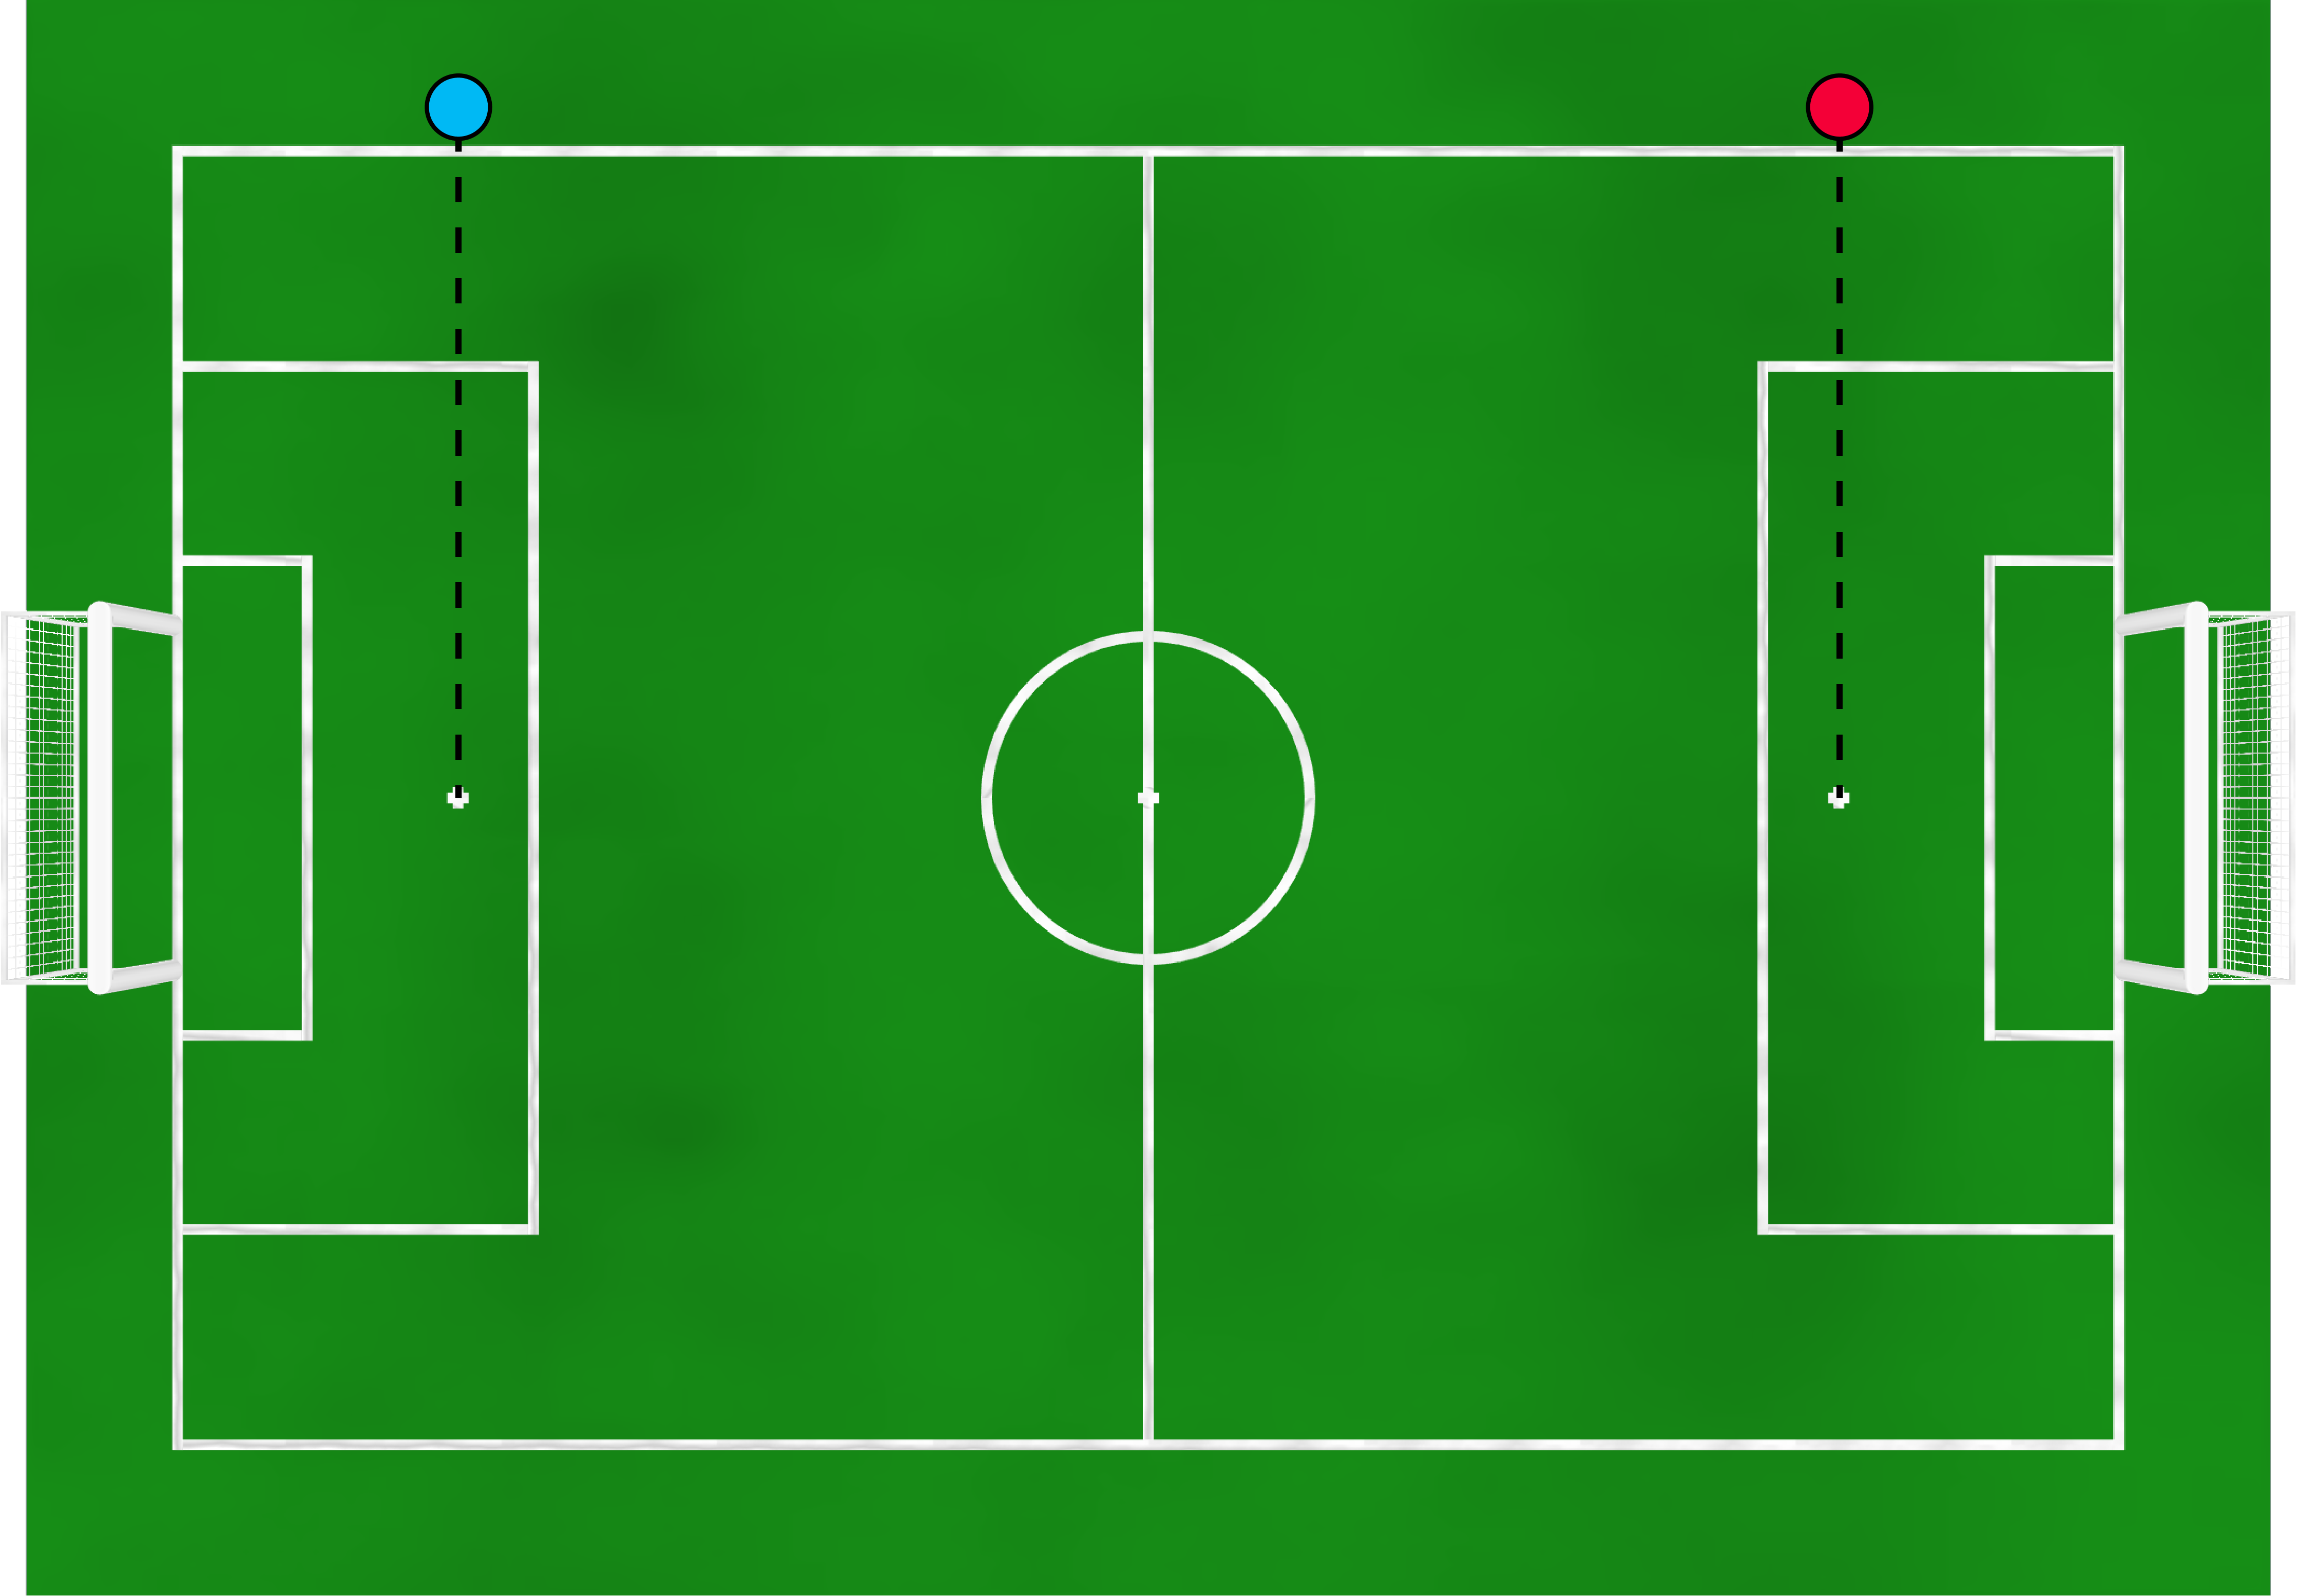
\includegraphics[width=\columnwidth]{figs/penalty_re-entry_points_2020.png}}
	\caption{For robots coming back from a standard removal penalty, re-entry points are inline with the penalty spot in their own half, on the sideline on the side away from the ball.}
	\label{fig:penalty_re-entry_points}
\end{figure}

When the robot is on the field again, the operator of the GameController will send the \emph{playing} signal to it.

\subsubsection{Forbidden Actions}

The following actions are forbidden, but not treated as penalties.
Each forbidden action specifies the actions to be taken by the referees.

\paragraph{Manual Interaction by Team Members}

Manual interaction with the robots, either directly or via some communications mechanism, is not permitted.

\paragraph{Locomotion Type}
\label{sec:locomotion_type}

Robots should clearly demonstrate bipedal walking similar to human walking. Other types of locomotion involving other parts than feet (crawling etc.) are strictly forbidden.
The head referee decides whether a robot's locomotion is appropriate. Robots using inappropriate locomotion types will be removed via ``Request for Pick-up'' until they are able to show appropriate locomotion.

\paragraph{Damage to the Field}
\label{sec:damage}

A robot that damages the field, or poses a threat to spectator safety, will be removed from the field for the remainder of the game.

\paragraph{Damage to the Robot}
\label{sec:damage_robot}

\cbp{The head referee decides whether a robot excessively damages itself and should remove it from the field via ``Request for Pick-up''. All referees are allowed to prevent robots from crashing to the ground by catching them beforehand and then laying them down gently.}
%Robots are not allowed to dive for the ball on purpose (\cf section \ref{sec:fallenrobots}).

\subsubsection{Illegal Positioning}
\label{sec:illegal_positioning}

A robot penalized under illegal position has the ``Illegal Position'' penalty applied. Illegally positioned robots are subject to the standard removal penalty (\cf Section~\ref{sec:removal_penalty}).
The head referee will call ``Illegal Position  \textless robot\textgreater''.

For simplicity, Illegal Positioning penalties during the \textit{set} state (for kick-off) do not count towards the incremental penalty count\footnote{Historically, the Illegal Positioning penalty only occurred during a kick-off, and other illegal actions were termed Illegal Defender. Illegal Positioning \& Defender have been merged, but the penalty count left unchanged.}.

Refer to Section~\ref{sec:inside_outside} for the definition of \textit{inside/outside} of a region of the field.

``Illegal Position'' shall be imposed if a robot is not inside its own half at the time the \textit{set} state starts. It will then be penalized and removed for 15 seconds. The centre line does not count as part of the own half for this penalty, \cbw{nor does the area inside the goal}.

\paragraph{Position for Kick-off}
If a robot is not inside its own half at the time the \textit{set} state starts, it will be penalized and removed for 15 seconds. The center line does not count as part of the own half for this penalty, \cbw{nor does the area inside the goal}.

\paragraph{Penalty Box, at all times}

Only \textit{three} players from the \textit{same} team can be in the \textit{same} penalty area at the same time\footnote{This means that if no goalkeeper is present, three field players may enter the penalty area to defend the goal.}. This means a total of 6 robots may in the same penalty box at the same time. \emph{This applies to all game states.}

A robot is within the penalty area if any part of its body is touching the ground inside the penalty box or touching one of its lines.  The penalty is applied when any additional players (whether field player or goalkeeper) enters the area. Note that if a player is pushed into the penalty area by an opponent, this robot will not be subject to removal, unless it fails to exit the area within 5 seconds (or 5 seconds \cbw{after} getting up if the pushing led to falling).

If an illegal defender kicks an own goal, the goal is scored for the opponent. If there is any doubt about whether a goal should count (\eg the illegal defender infraction is called, but the robot scores the own goal immediately afterwards, before it is removed) then the decision shall be against the infringing robot.

\paragraph{Center Circle, during Kick-off}

The penalty is applied to defensive players that enter the centre circle after a kick-off before the ball is in play (\cf Section~\ref{sec:kick-off}).

\paragraph{Defender Encroachment, during Free-kick}

If a robot of the offending team does enter or not attempt to leave the \FreeKickRadius area around the ball after a Free Kick (\cf Section~\ref{sec:free_kick}) was called, ``Illegal Position'' is called. This rule does not apply for the goalkeeper robot within its own penalty area. Note that the referee should not look for exact distances and rather penalize only those robots who clearly violate this rule. As a guideline, the robots of the offending team should clear the ball within 10 seconds.

\paragraph{Penalty Box, during Free-kick}

If a robot that enters the relevant penalty box during a penalty kick, except for the goalkeeper (defending team) and one robot of the attacking team, ``Illegal Position'' is called.


\subsubsection{Motion in Set}
\label{sec:motion_in_set}

Robots may not exit the \textit{set} state until either the referee's whistle is detected or a GameController \textit{playing} signal has been received.
The head referee will call ``Motion in Set \textless robot\textgreater''.
The offending robot is penalized \textbf{in-place} on the field. It will then be unable to move until it receives the GameController \textit{playing} signal. Motion in Set penalties do not follow the standard removal procedure, and hence do not count towards the incremental penalty count.

\subsubsection{Fallen or Inactive Robots}
\label{sec:fallenrobots}

If a robot falls during the game, it should start executing a getup action within 5 seconds. If it does not commence a get up action within 5 seconds, it will be penalized and removed for \StandardPenaltyTime.
A robot which is unable to autonomously stand up within 20 seconds after a fall \cbw{and be at least 10 seconds upright} will be penalized and removed for \StandardPenaltyTime. 
In both cases, the head referee will call ``Fallen Robot  \textless robot\textgreater''.

The goal keeper, inside its own penalty area, is the only robot permitted to `dive' (that is deliberately fall in a way that might cause its torso, arms or hands) to intercept the ball. In all other cases, the robot should be programmed to attempt to remain upright -- that is, supported by its feet.

A robot that has ceased activity for 10 seconds or has turned off will be removed and penalized for 45 seconds.
The head referee will call ``Inactive Robot  \textless robot\textgreater''.
A robot is active if it performs at least one of the following:
\begin{enumerate}
	\item The robot walks in any direction, or turns.
	\item The robot searches for the ball, or is looking at the ball.
\end{enumerate}

Fallen/Inactive Robot penalties do not follow the standard removal procedure, and hence do not count towards the incremental penalty count.

\textbf{Note:} The intention of this rule is not to penalize robots simply for being stationary -- provided they are not `asleep' and have not `crashed'.

\subsubsection{Local Game Stuck}
\label{sec:pen_local_game_stuck}

When Local Game Stuck is called, the nearest robot to the ball will be penalized and removed for 45 seconds. Local Game Stuck penalties do not follow the standard removal procedure, and hence do not count towards the incremental penalty count.

\subsubsection{Ball Holding}
\label{sec:ball_holding}

The goal keeper is allowed to hold the ball for up to 10 seconds as long as it has one foot inside in its own penalty area.  In all other cases (except those noted in Section~\ref{sec:situations_no_ball_holding}), robots are allowed to hold the ball for up to 3 seconds. Holding the ball for longer than this is not allowed.
The head referee will call ``Ball Holding \textless robot\textgreater'', and the robot removed under the standard removal penalty.
The ball should be removed from the possession of the robot and placed where the penalty occurred.
If the robot that held the ball has moved the ball before the robot can be removed, the ball shall be replaced where the penalty occurred.
This applies to accidental goals.

\textbf{Example.} A robot holds the ball, and before the referees can remove the robot, it shoots the ball into the goal. The goal will not be counted and the ball will be replaced where the penalty occurred,

%A robot which does not leave enough open space around the ball will be penalized as ``Ball Holding'' if that situation continues more than 3 seconds.
A robot must leave enough open space around the ball. The occupation of the ball is judged using the convex hull of the projection of the robot's body onto the ground. ``Enough open space'' means that at least the half of the ball is not covered by the convex hull. It is not important whether the robot actually touches the ball.

\begin{figure}[t]
\centerline{\begin{tabular}{ll}
a) & b) \\
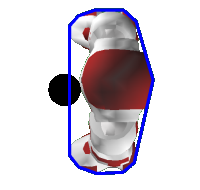
\includegraphics[scale=0.7]{figs/holding1} &
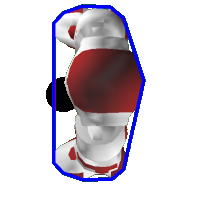
\includegraphics[scale=0.7]{figs/holding4}
\end{tabular}}

\caption{Examples for ``Ball Holding''. The black circle is the ball, the blue polygon visualizes the convex hull of the robot's projection onto the ground and the red area shows the occupied portion of the ball. Situations a) is legal, whereas b) violates the rule.}
\label{fig:holding}
\end{figure}

Intentional continual holding is prohibited even if each individual holding time does not continue for up to the time limit. In general, robots should release the ball for approximately as long as they were holding it to reset the clock. Without a sufficient release, the continual holding is regarded as a continuous hold from the very beginning and the holding rule is strictly applied.


\paragraph{Exceptions to the Ball Holding Rules}
\label{sec:situations_no_ball_holding}

The following defines situations where ball holding does not apply:

\begin{enumerate}
\item Ball holding may not occur when the ball becomes stuck between a robot's legs.  In such a situation, the head referee should call `clear ball' and an assistant referee should remove the ball and place the ball approximately where it was before it became stuck.
\item Ball holding may not occur when a robot falls on a ball.  The robot will either get-up and hence free the ball, or the robot should be removed under the Fallen Robot rule.
\end{enumerate}

\subsubsection{Player Stance}
\label{sec:player_stance}
\cbw{In order to intercept kicked balls the robots are} allowed to go into a wide stance as long as they come back to a normal stance within 5 seconds \cbw{and do not excessively damage the robots}\footnote{\cbw{``excessively'' is decided by the head referee in order to limit damages to robots}}. \\
Robots are not allowed to stay in a stance that is wider than the width of the robot's shoulders for more than 5 seconds. Staying in a wide stance for longer than 5 seconds will result in the standard removal penalty. \\
If the robot has fallen down, it must start getting up within 5 seconds. 

\subsubsection{Player Pushing}
\label{sec:player_pushing}

\emph{Pushing} is a forceful contact with another robot\footnote{This includes robots that are getting up or lie on the field.}, \ie, enough to destabilize it, and is not allowed. In the following, exceptions to this rule are specified in more detail.
The head referee will call ``Pushing \textless robot\textgreater''.

\cbw{Pushing may occur \textbf{between any robots}, i.e. also between team mates.}

If the ball moves significantly as the result of pushing, then it should be replaced to where it was at the time of the infraction.

A Pushing Free Kick is awarded against the robot penalized for pushing if the robot is near the ball (approximately within 0.5m of the ball).

\paragraph{Exceptions to the Pushing Rules}
\label{sec:situations_no_pushing}

The following define situations where pushing does not apply:

\begin{enumerate}
  \item A stationary robot cannot be penalized for pushing, including a robot that is kicking, provided that the ball was close enough where a kick could have succeeded at the start of the kick motion.
  \item A robot currently getting up cannot be penalized for pushing.
  \item The goal keeper cannot be penalized for pushing while looking at or chasing the ball in it's own penalty area.
  \item Front to front contact between robots with the ball between them does not constitute pushing.
  \item Any robot proceeding to the ball whose side (\ie arm, shoulder etc.) makes contact with another robot cannot be called for pushing, Even if the second robot is not proceeding to the ball.
  \item A robot pushed by another robot can not simultaneously be called for pushing itself.
\end{enumerate}

\subsubsection{Playing with Arms/Hands}
\label{sec:hand_ball}

Playing with arms/hands occurs when a field player moves its arms/hands to touch the ball (except during a fall or get-up). A robot playing with arms/hands will be subject to the standard removal penalty and the ball will be replaced at the point where it contacted the arms/hands of the offending robot. If an own goal is scored as a result, the goal should count and the player should not be penalized.

Accidental playing with arms/hands when a robot falls or executes a get-up routine will not be penalized. 
If the ball goes out of play in this case, normal kick-in rules will apply (\cf Section~\ref{sec:kick_in}). 
Goals resulting from a ball contact with the arms/hands during a fall or get-up do not count and result in a Goal Kick (\cf Section~\ref{sec:free_kick}) as if the ball went over the goal line next to the goal.

\subsubsection{Leaving the Field}
\label{sec:leaving_field}

A robot that intends to leave the \TotalWidth $\times$ \TotalLength carpeted area will be subject to the standard removal penalty (\cf Section~\ref{sec:removal_penalty}).
The head referee will call ``Leaving the Field \textless robot\textgreater''.

Additionally, a robot will also be subject to the standard removal penalty where:
\begin{itemize}
\item the robot walks into the goal posts or goal net for more than 5 seconds, this includes robots that are stuck on the goal posts and unable to free themselves
\item the robot's finger become entangled in the net (without any time constraint).
\end{itemize}

\subsubsection{Jamming}
\label{sec:jamming}
During the match, any robot shall never jam the communication and the sensor systems of the opponents:

\begin{description}

\item[Wireless communication.] Each robot is only allowed to send a limited number of UDP messages that have to comply with a predefined format (\cf Section~\ref{sec:wireless}). If a robot uses a different protocol or sends too many messages over a couple of seconds in a game, it will be disqualified for that game. If a team violates this rule in multiple games, disqualification from the tournament (including technical challenges) as well as an entry in the penalty list will be the consequence. Except for the wireless cards and the access points provided by the organizers of the competition, nobody close to the field is allowed using 2.4~GHz radio equipment (including cellular phones and/or Bluetooth devices).

\item[Whistle interference.] Both the teams and the audience shall avoid intentionally confusing the robots by producing similar sounds to the game whistle.

\item[Acoustic communication.] If acoustic communication is used by both teams, they shall negotiate before the match how they can reduce interference. If only one team uses acoustic communication, the robots of the other team shall avoid producing any sound. In addition, both the teams and the audience shall avoid intentionally confusing the robots by producing similar sounds to those used for communication.

\item[Infrared communication.] If infrared communication is used by both teams, they shall negotiate before the match how they can reduce interference (if at all). Both the teams and the audience shall avoid confusing the robots by producing similar infrared signals to those used for communication.

\item[Visual perception.] The use of flashlights is not allowed during the games.  However, flash photography from the audience is allowable as long as the head referee believes the purpose of the flash is not to jam any of the robots.

\end{description}

\subsection{Judgment}
\label{sec:judgment}
The referees are the only persons permitted on the carpeted area (\ie the field and the border area).

\cbp{The local team of an arena has to provide the referees. The number of referees depends on local regulations and can be reduced to a head referee and an operator of the GameController.}

\cbp{All referees are allowed to prevent robots from crashing to the ground by catching them beforehand and then laying them down gently!}

\subsubsection{Head Referee}
\label{sec:head_referee}

The head referee is in charge of the game. Any decision of the head referee is valid. The head referee's decision is final and can not be changed afterwards, even by video proof. There is no discussion about decisions during the game, neither between the assistant referees and the head referee, nor between the audience/spectators or the teams and the head referee.

\cbp{The head referee also decides whether a robot excessively damages itself and should be removed from the field (\cf Section~\ref{sec:damage})}.

The head referee announces decisions by a clear loud call, and (as required) whistle sound.
The whistle, or where there is no whistle the first verbal word of the referees calls, defines the point in time at which the decision is made.
The referees should make efforts to use consistent and clear calls, and it is preferable for referees to use the calls as specified in these rules\footnote{The calls specified in these rules are detailed in English. With the agreement of the teams, the referees may use suitable calls in any language. The exception to this are technical challenge(s) that depends on the calls as specified.}.
The intention of specifying the referee calls is for clarity and consistency across games.

Where a whistle is required, the head referee first whistles and then announces the reason for the whistle.
The head referee may choose to use any normal sports whistle.
Each whistle sound should be short and not too loud.
The head referee must \textit{only} sound the whistle in circumstances described in these rules.
There are three circumstances when the whistle is sounded, Kick-off~(\cf Section~\ref{sec:kick-off}), a goal~(\cf Section~\ref{sec:goal}), and ending a half of gameplay~(\cf Section~\ref{sec:game_struct}).

The head referee should avoid handling the ball (except for placing a ball for a kick-off), and avoid handling the robots.
Their duty is to monitor and adjudicate the game.
The head referee should only handle robots and the ball if absolutely necessary to expedite gameplay or removal of penalized robots, where the assistant referees are otherwise occupied, are too far away \cbw{or had to be dropped due to local regulations.}

\subsubsection{Assistant Referees}
\label{sec:assist_referee}
The, \cbw{in the ideal case}, two assistant referees handle the robots and the ball. They start the robots if they are not using the GameController, they move the robots, if a manual placement is needed, they take the robots out when they are penalized, and they put the robots in again. An assistant referee will also replace the ball when it goes off the field or becomes stuck between a players feet.

\cbp{If a team requests to pick up a robot, an assistant referee will pick it up and put it on the sideline. Also the assistant, on behalf of the teams, can do hardware changes to robots on the sideline, \ie reboot it or change and secure the battery.}

The assistant referees can \textit{indicate} violations against the rules committed by robots to the head referee, so that the head referee can decide whether to penalize a certain robot or not. Assistant referees should only enter the field to execute a decision made by the main referee \cbw{or to catch a falling robot}.

\subsubsection{Operator of the GameController}
\label{sec:gameControllerOp}
The operator of the GameController sits at a PC outside the playing area.
As with the head referee, the operator should make efforts to use consistent and clear calls.
They will signal any change in the game state to the robots via the wireless as they are announced by the head referee.
Note that for both kick-offs and goals, the moment of whistling is determining, not the verbal announcement of the head referee.
The operator will also inform the assistant referees when a timed penalty is over and a robot has to be placed back on the field.
They should announce when the ball is in play on kick-off by stating ``Ball Free'', if the \KickOffBallFreeTime time period has elapsed in the playing state.
They are also responsible for keeping the time of each half (\ie, they stop the clock after a global game stuck, and continues it at the kick-off).
They should count aloud the remaining seconds in a half once the time remaining is 5 seconds or less.
Finally, they should repeat the calls of the head referee to make sure it was heard correctly.

\subsubsection{Referees During the Match}

The head referee and the assistant referees should wear clothing and socks \emph{of black or dark blue colour} (blue jeans are acceptable) and avoid reserved colours for the ball, the goals, and player markings in their clothing. They may enter the field in particular situations, \eg, to remove a robot when applying a penalty \cbw{or to catch a falling robot}. They should avoid interfering with the robots as much as possible.

\subsubsection{A Remark on Artificial Landmarks}
\label{sec:judgment:landmarks}

The head referee may decide at any point before or during a game to relocate any objects around the field, or direct persons to another position around the field.

The intent of using same-coloured goals is to remove artificial landmarks.
Robots should be able to localize with the SPL field and its ``normal'' surroundings.
Introducing new team-specific artificial landmarks is against the spirit and intention of the league's progress.
The application of this rule needs to be well considered and should be reserved for situations which seem constructed by one team or another, but will ultimately be the head referee's decision alone.

\newpage

\subsection{Technical Field Drawings}
\label{apx:technical-drawing}
\centerline{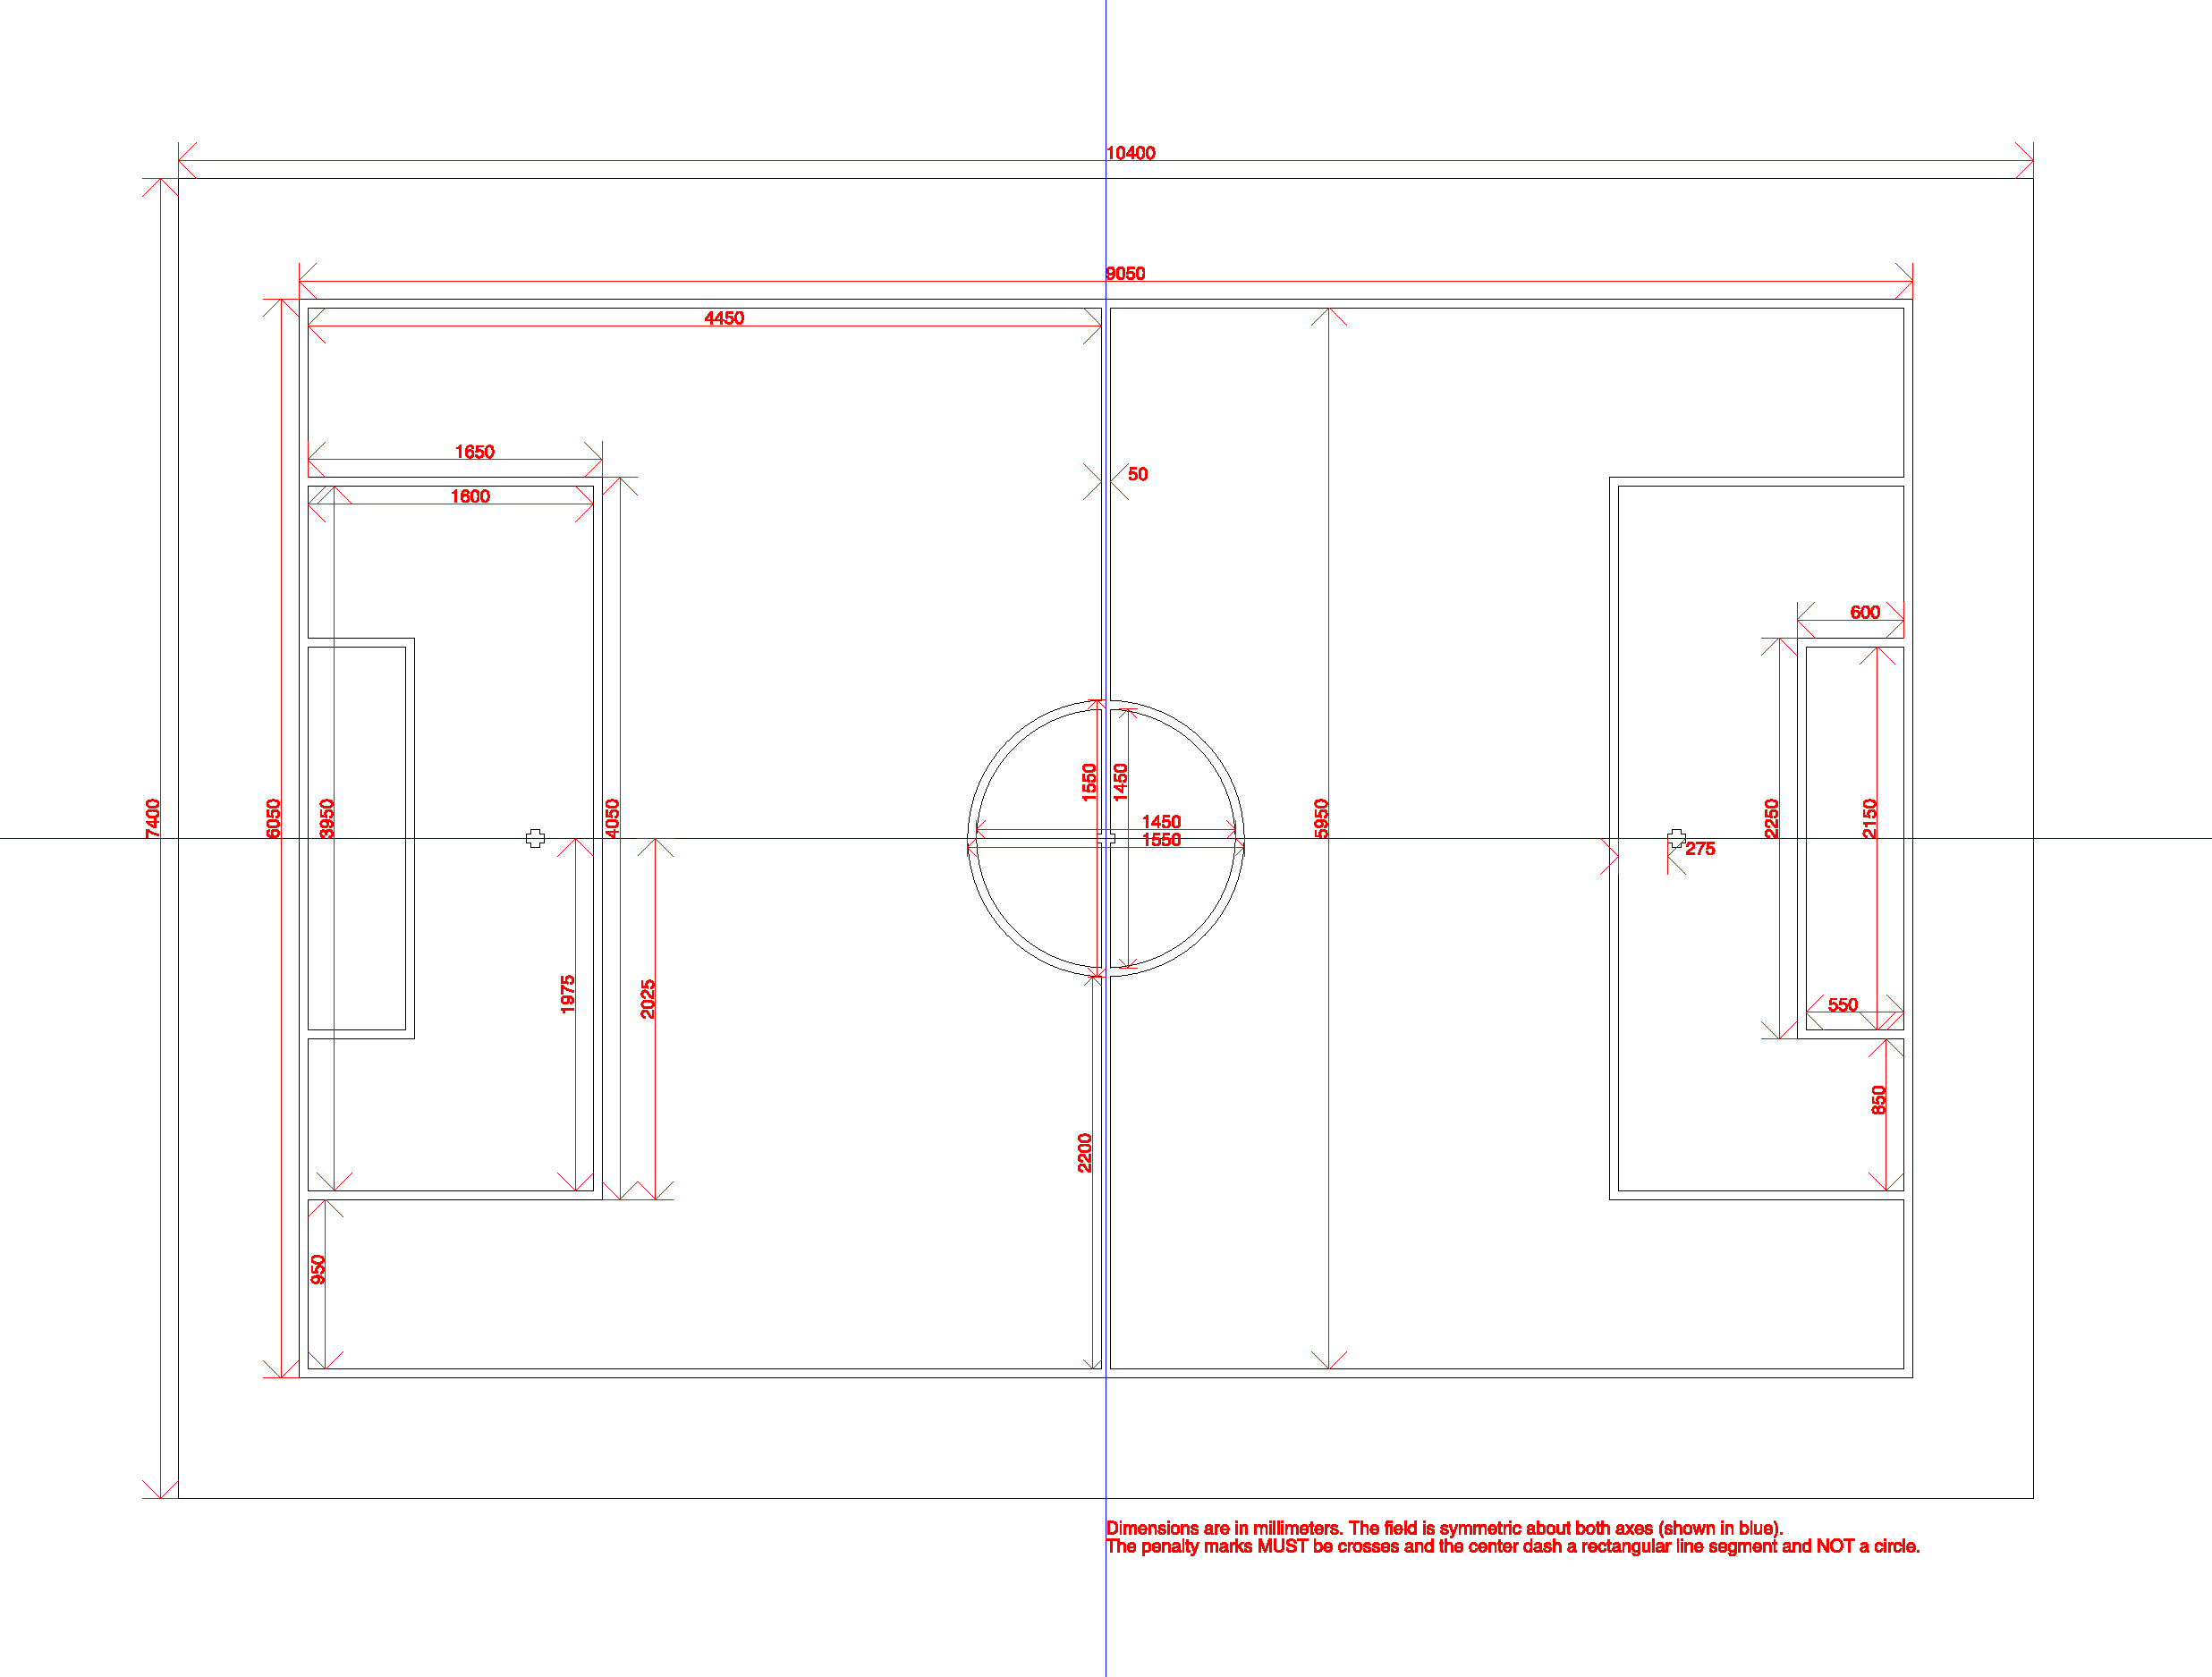
\includegraphics[angle=90,origin=c,width=\columnwidth]{figs/fieldDimensions2020_technical.pdf}}

\clearpage
\centerline{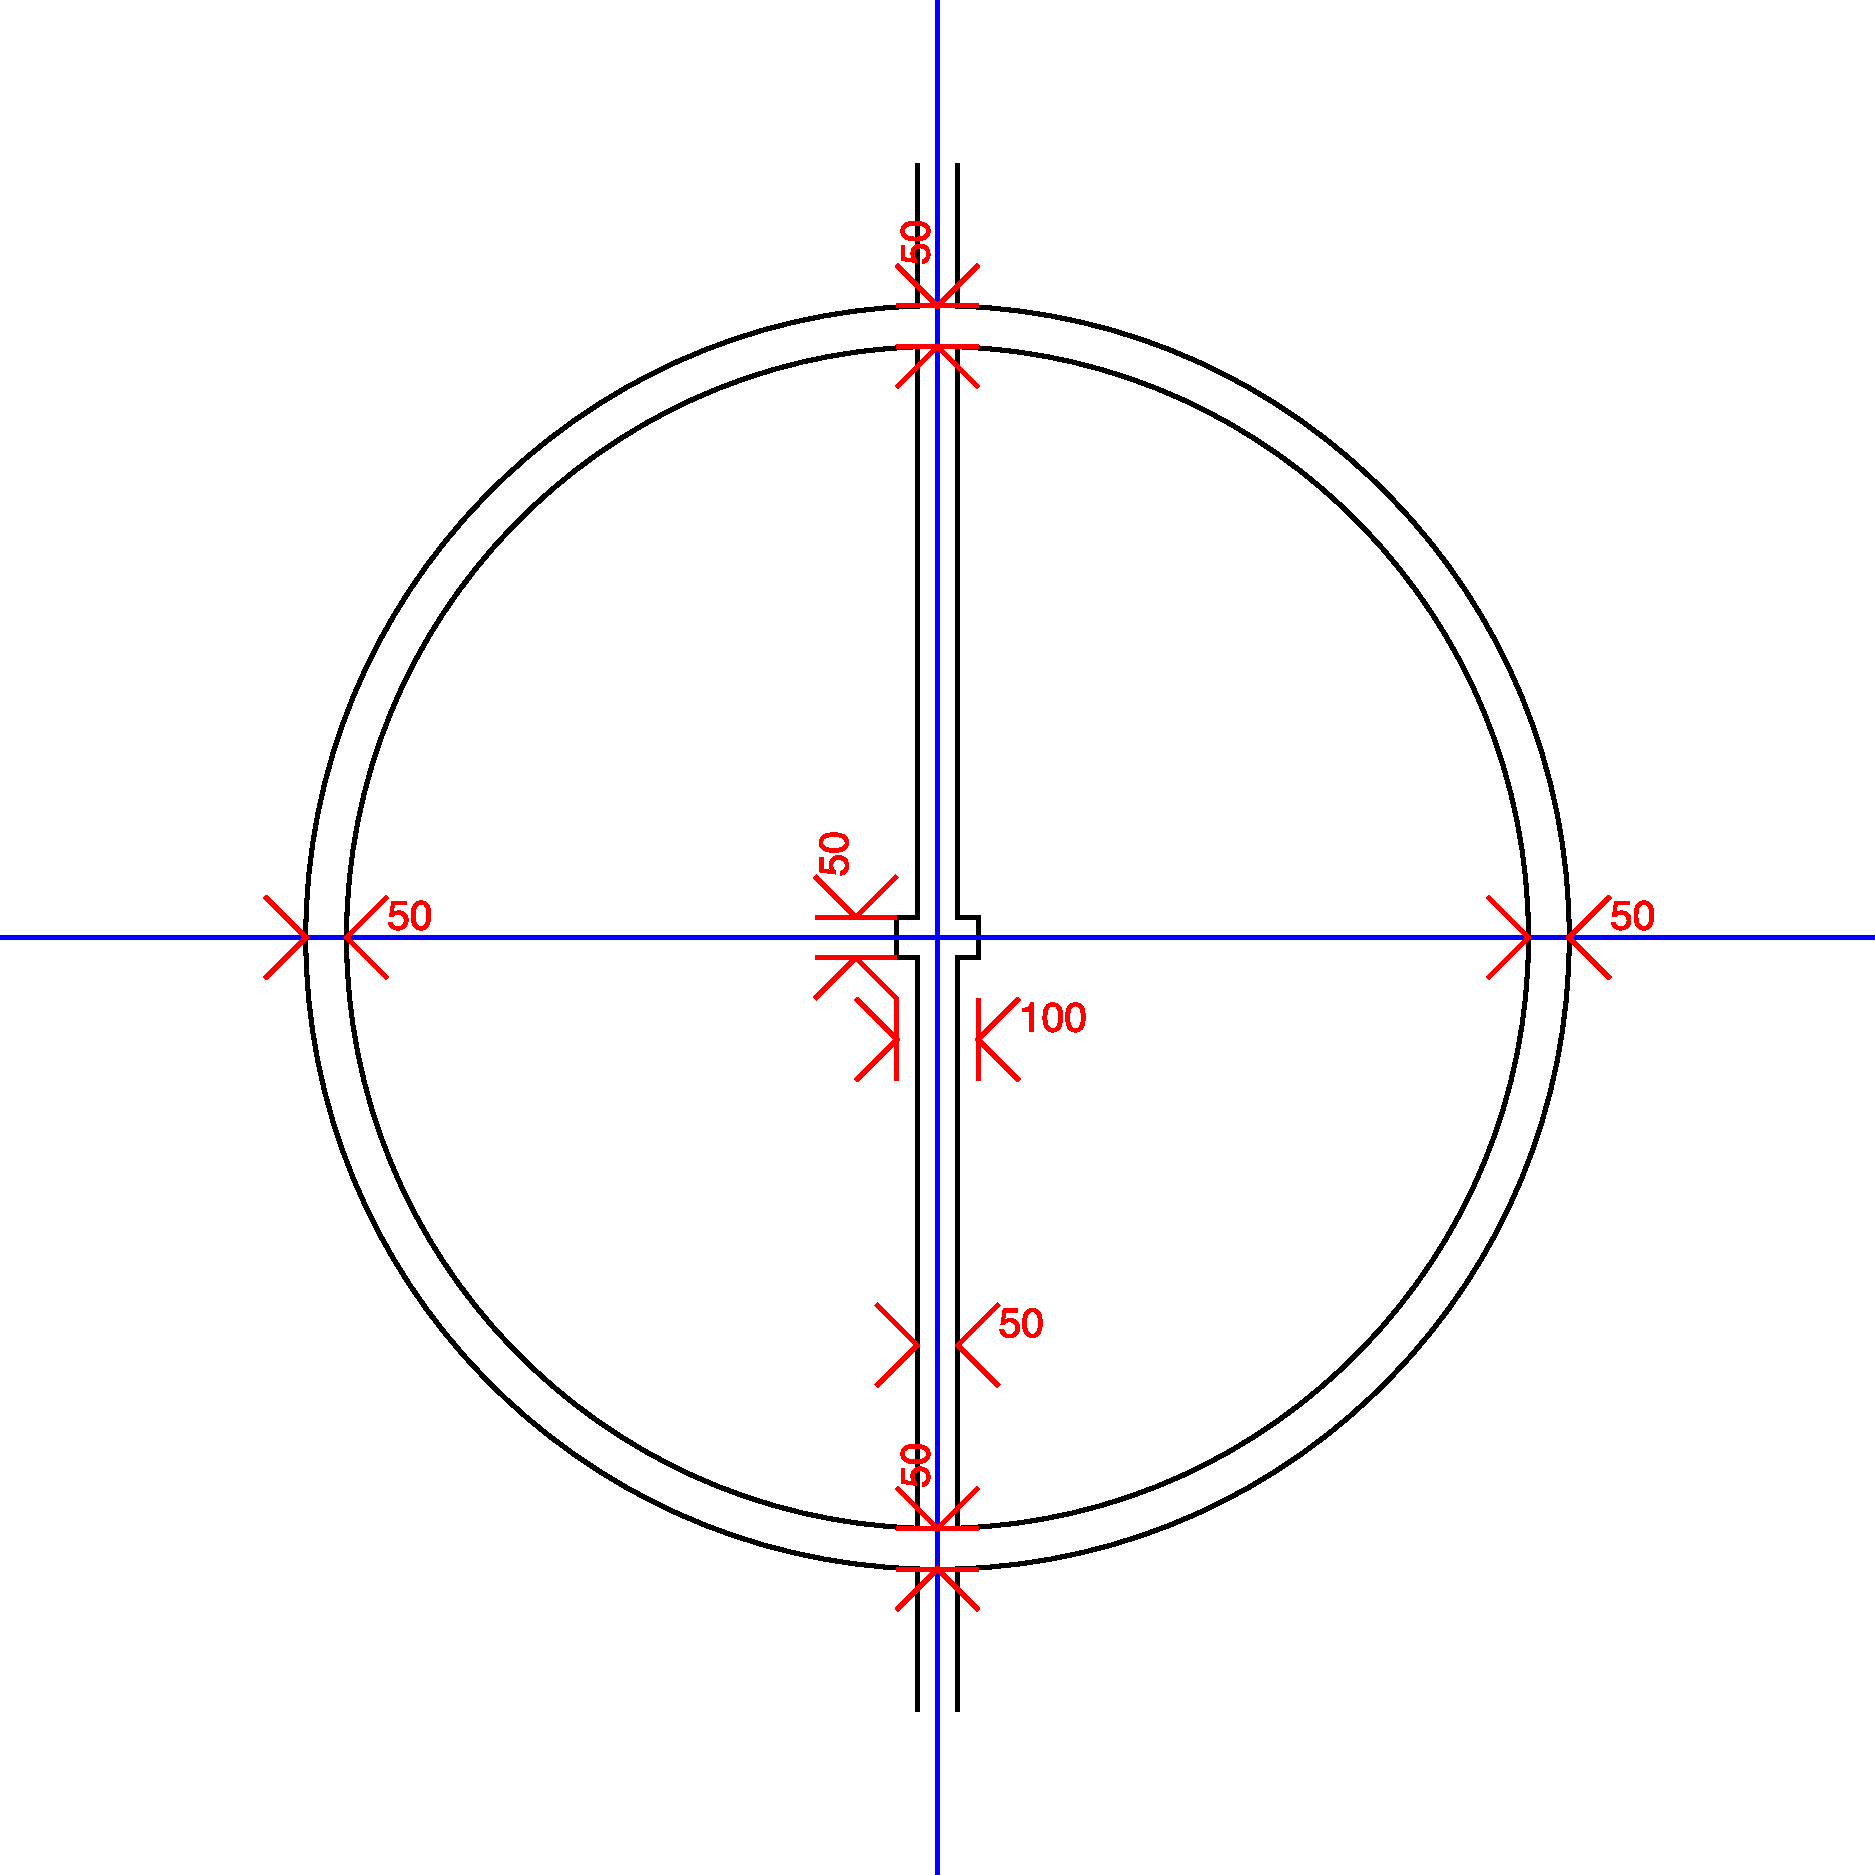
\includegraphics[angle=90,origin=c,width=0.5\columnwidth]{figs/fieldDimensions2020_technical_cc.pdf}}

\centerline{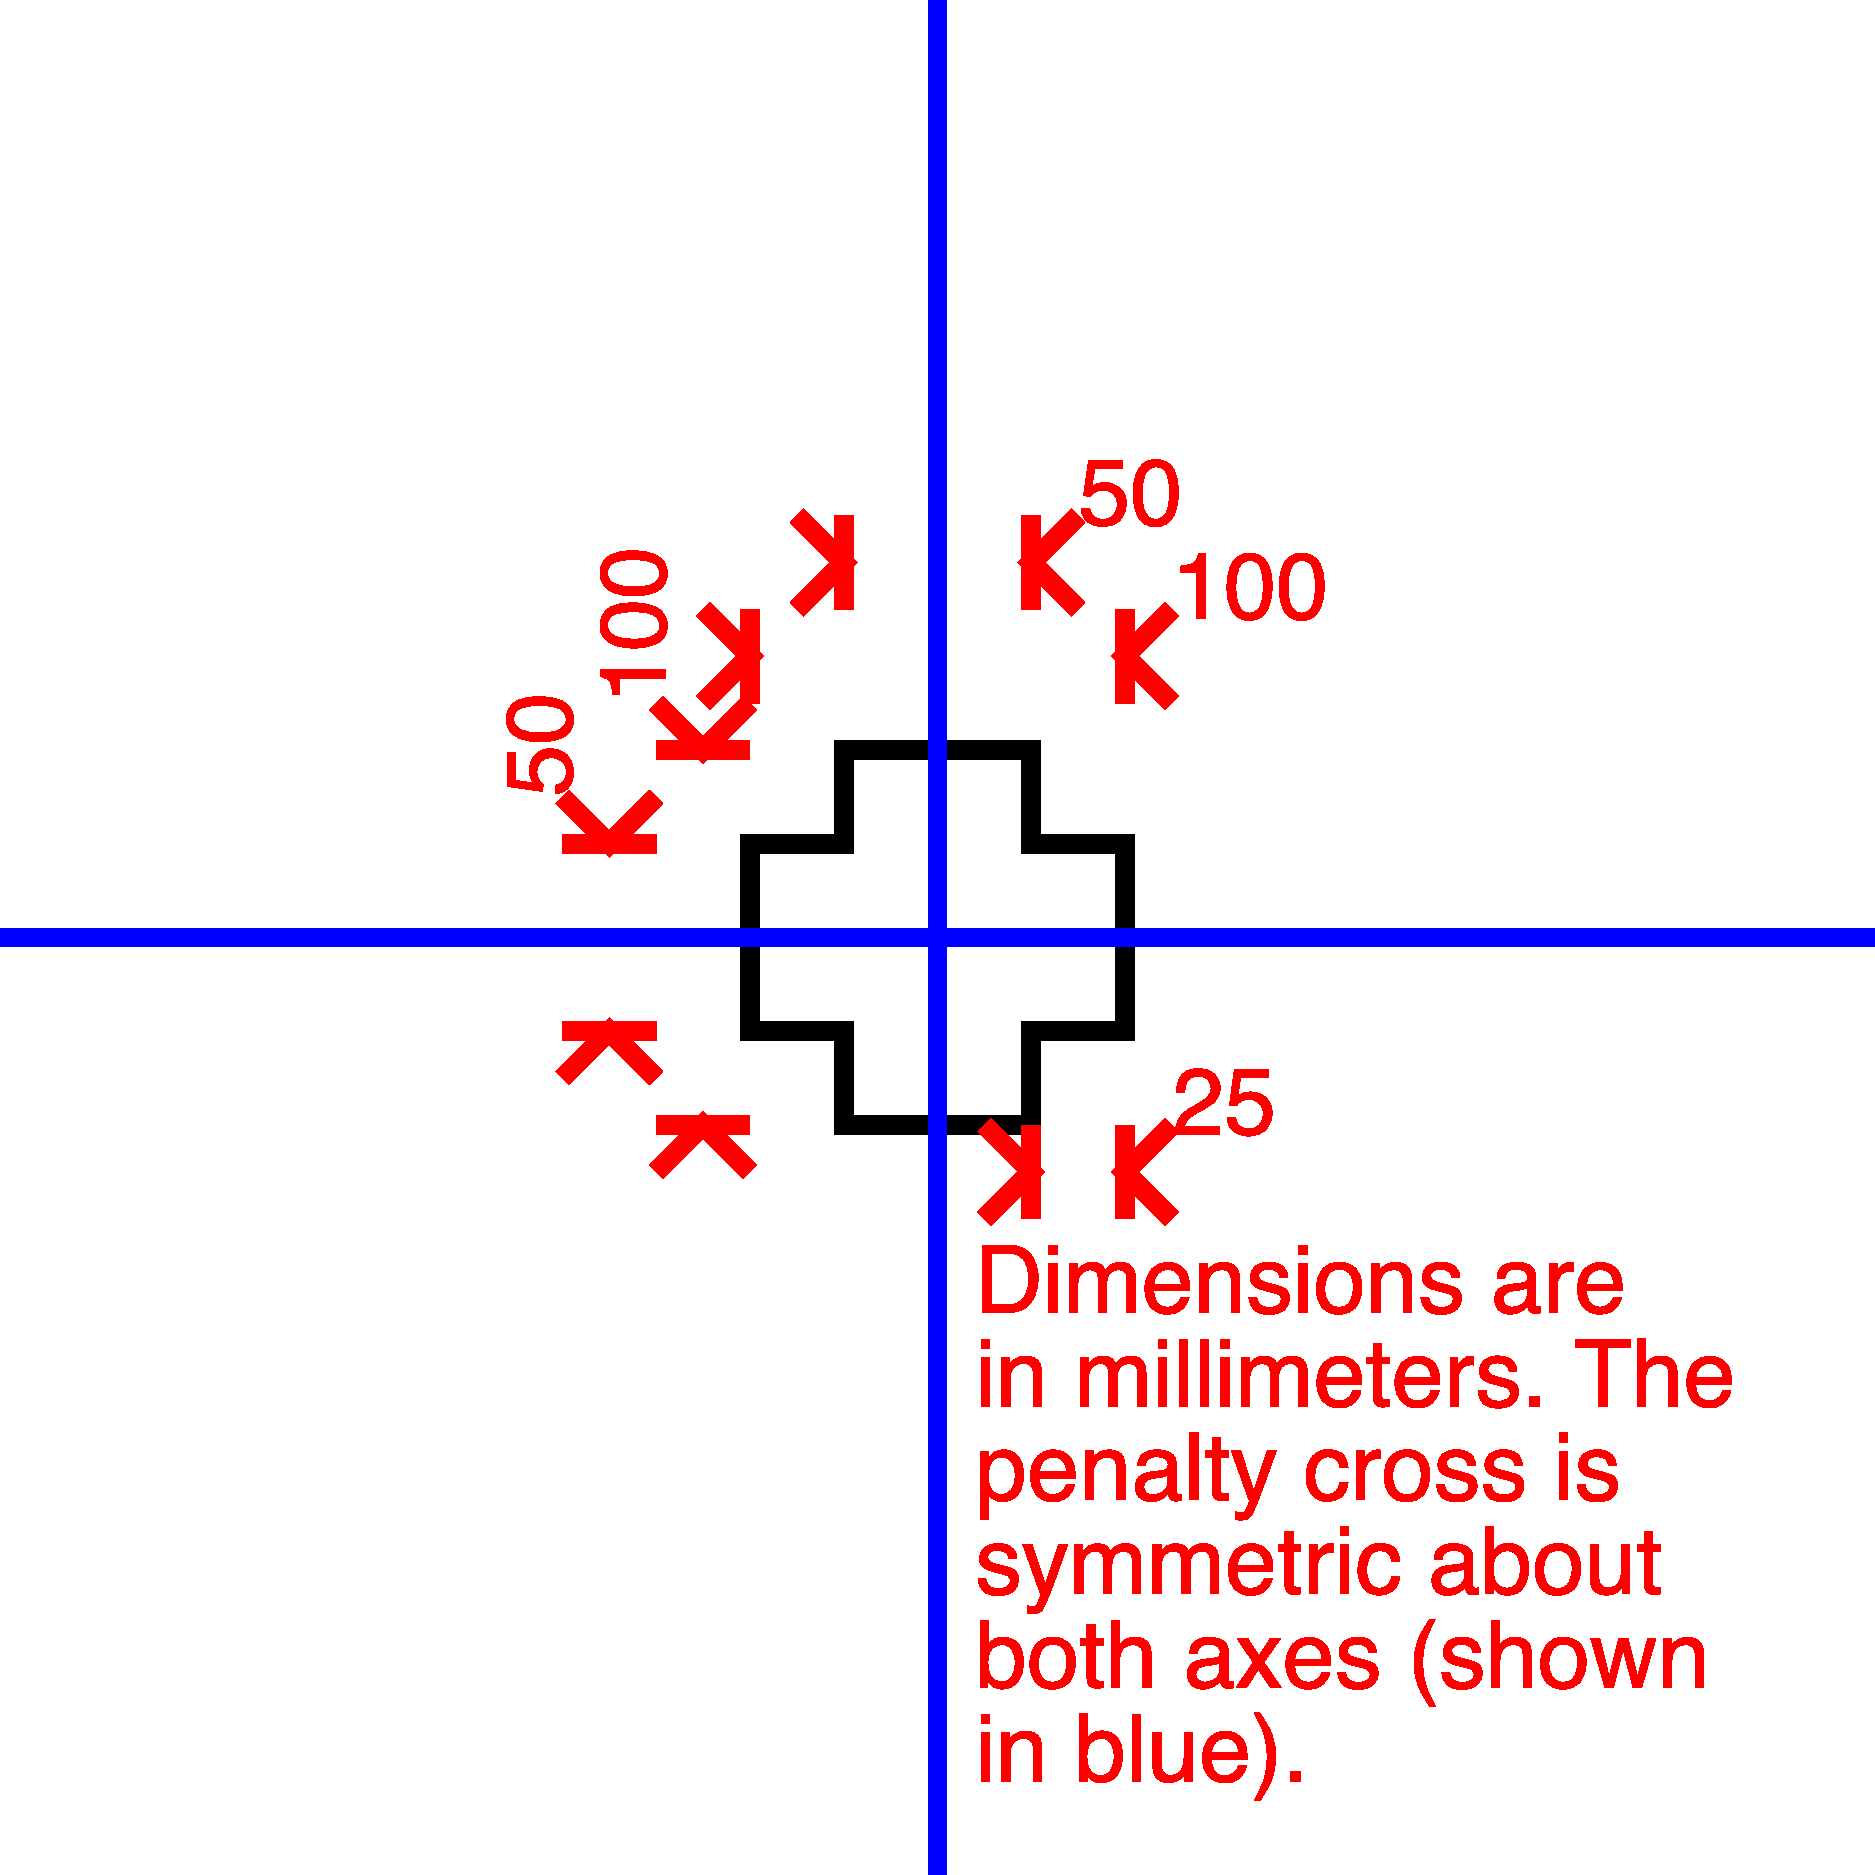
\includegraphics[origin=c,width=0.5\columnwidth]{figs/fieldDimensions2020_technical_pc.pdf}}
